% **************************************************************************************************************
% A Classic Thesis Style
% An Homage to The Elements of Typographic Style
%
% Copyright (C) 2017 André Miede and Ivo Pletikosić
%
% If you like the style then I would appreciate a postcard. My address
% can be found in the file ClassicThesis.pdf. A collection of the
% postcards I received so far is available online at
% http://postcards.miede.de
%
% License:
% This program is free software; you can redistribute it and/or modify
% it under the terms of the GNU General Public License as published by
% the Free Software Foundation; either version 2 of the License, or
% (at your option) any later version.
%
% This program is distributed in the hope that it will be useful,
% but WITHOUT ANY WARRANTY; without even the implied warranty of
% MERCHANTABILITY or FITNESS FOR A PARTICULAR PURPOSE.  See the
% GNU General Public License for more details.
%
% You should have received a copy of the GNU General Public License
% along with this program; see the file COPYING.  If not, write to
% the Free Software Foundation, Inc., 59 Temple Place - Suite 330,
% Boston, MA 02111-1307, USA.
%
% PLEASE SEE ALSO THE AUTHORS' NOTE REGARDING THIS LICENSE
% IN THE DOCUMENTATION (ClassicThesis.pdf --> Chapter 1 / Chapter01.tex)
% **************************************************************************************************************
\RequirePackage{silence} % :-\
    \WarningFilter{scrreprt}{Usage of package `titlesec'}
    %\WarningFilter{scrreprt}{Activating an ugly workaround}
    \WarningFilter{titlesec}{Non standard sectioning command detected}
\documentclass[ twoside,openright,titlepage,numbers=noenddot,headinclude,%1headlines,% letterpaper a4paper
                footinclude=true,cleardoublepage=empty,abstractoff, % <--- obsolete, remove (todo)
                BCOR=5mm,paper=a4,fontsize=11pt,%11pt,a4paper,%
                ngerman,american,%
                ]{scrreprt}

%********************************************************************
% Note: Make all your adjustments in here
%*******************************************************
% ****************************************************************************************************
% classicthesis-config.tex
% formerly known as loadpackages.sty, classicthesis-ldpkg.sty, and classicthesis-preamble.sty
% Use it at the beginning of your ClassicThesis.tex, or as a LaTeX Preamble
% in your ClassicThesis.{tex,lyx} with % ****************************************************************************************************
% classicthesis-config.tex
% formerly known as loadpackages.sty, classicthesis-ldpkg.sty, and classicthesis-preamble.sty
% Use it at the beginning of your ClassicThesis.tex, or as a LaTeX Preamble
% in your ClassicThesis.{tex,lyx} with % ****************************************************************************************************
% classicthesis-config.tex
% formerly known as loadpackages.sty, classicthesis-ldpkg.sty, and classicthesis-preamble.sty
% Use it at the beginning of your ClassicThesis.tex, or as a LaTeX Preamble
% in your ClassicThesis.{tex,lyx} with \input{classicthesis-config}
% ****************************************************************************************************
% If you like the classicthesis, then I would appreciate a postcard.
% My address can be found in the file ClassicThesis.pdf. A collection
% of the postcards I received so far is available online at
% http://postcards.miede.de
% ****************************************************************************************************


% ****************************************************************************************************
% 0. Set the encoding of your files. UTF-8 is the only sensible encoding nowadays. If you can't read
% äöüßáéçèê∂åëæƒÏ€ then change the encoding setting in your editor, not the line below. If your editor
% does not support utf8 use another editor!
% ****************************************************************************************************
\PassOptionsToPackage{utf8}{inputenc}
  \usepackage{inputenc}

% ****************************************************************************************************
% 1. Configure classicthesis for your needs here, e.g., remove "drafting" below
% in order to deactivate the time-stamp on the pages
% (see ClassicThesis.pdf for more information):
% ****************************************************************************************************
\PassOptionsToPackage{
  drafting=false,    % print version information on the bottom of the pages
  tocaligned=false, % the left column of the toc will be aligned (no indentation)
  dottedtoc=false,  % page numbers in ToC flushed right
  parts=true,       % use part division
  eulerchapternumbers=true, % use AMS Euler for chapter font (otherwise Palatino)
  linedheaders=false,       % chaper headers will have line above and beneath
  floatperchapter=true,     % numbering per chapter for all floats (i.e., Figure 1.1)
  listings=true,    % load listings package and setup LoL
  subfig=true,      % setup for preloaded subfig package
  eulermath=false,  % use awesome Euler fonts for mathematical formulae (only with pdfLaTeX)
  beramono=true,    % toggle a nice monospaced font (w/ bold)
  minionpro=false   % setup for minion pro font; use minion pro small caps as well (only with pdfLaTeX)
}{classicthesis}


% ****************************************************************************************************
% 2. Personal data and user ad-hoc commands
% ****************************************************************************************************
\newcommand{\myTitle}{Procedural Content Generation in Computer Games\xspace}
\newcommand{\mySubtitle}{Level Generation for Angry Birds using Genetic Algorithms\xspace}
\newcommand{\myDegree}{Grado en Ingeniería Informática\xspace}
\newcommand{\myName}{Laura Calle Caraballo\xspace}
\newcommand{\myProf}{Juan Julián Merelo Guervós\xspace}
\newcommand{\myOtherProf}{.\xspace}
\newcommand{\mySupervisor}{.\xspace}
\newcommand{\myFaculty}{Escuela Técnica Superior de Ingenierías Informática y de Telecomunicación\xspace}
\newcommand{\myDepartment}{Put data here\xspace}
\newcommand{\myUni}{Universidad de Granada\xspace}
\newcommand{\myLocation}{Granada\xspace}
\newcommand{\myTime}{\today\xspace}
\newcommand{\myVersion}{version0}

% ********************************************************************
% Setup, finetuning, and useful commands
% ********************************************************************
\newcounter{dummy} % necessary for correct hyperlinks (to index, bib, etc.)
\newlength{\abcd} % for ab..z string length calculation
\providecommand{\mLyX}{L\kern-.1667em\lower.25em\hbox{Y}\kern-.125emX\@}
\newcommand{\ie}{i.\,e.}
\newcommand{\Ie}{I.\,e.}
\newcommand{\eg}{e.\,g.}
\newcommand{\Eg}{E.\,g.}
% ****************************************************************************************************


% ****************************************************************************************************
% 3. Loading some handy packages
% ****************************************************************************************************
% ********************************************************************
% Packages with options that might require adjustments
% ********************************************************************
%\PassOptionsToPackage{ngerman,american}{babel}   % change this to your language(s), main language last
% Spanish languages need extra options in order to work with this template
%\PassOptionsToPackage{spanish,es-lcroman}{babel}
    \usepackage{babel}

\usepackage{csquotes}
\PassOptionsToPackage{%
  %backend=biber,bibencoding=utf8, %instead of bibtex
  backend=bibtex8,bibencoding=ascii,%
  language=auto,%
  style=numeric-comp,%
  %style=authoryear-comp, % Author 1999, 2010
  %bibstyle=authoryear,dashed=false, % dashed: substitute rep. author with ---
  sorting=nyt, % name, year, title
  maxbibnames=10, % default: 3, et al.
  %backref=true,%
  natbib=true % natbib compatibility mode (\citep and \citet still work)
}{biblatex}
    \usepackage{biblatex}

\PassOptionsToPackage{fleqn}{amsmath}       % math environments and more by the AMS
  \usepackage{amsmath}

% ********************************************************************
% General useful packages
% ********************************************************************
\PassOptionsToPackage{T1}{fontenc} % T2A for cyrillics
  \usepackage{fontenc}
\usepackage{textcomp} % fix warning with missing font shapes
\usepackage{scrhack} % fix warnings when using KOMA with listings package
\usepackage{xspace} % to get the spacing after macros right
\usepackage{mparhack} % get marginpar right
%\usepackage{fixltx2e} % fixes some LaTeX stuff --> since 2015 in the LaTeX kernel (see below)
% \usepackage[latest]{latexrelease} % emulate newer kernel version if older is detected
\PassOptionsToPackage{printonlyused,smaller}{acronym}
  \usepackage{acronym} % nice macros for handling all acronyms in the thesis
  %\renewcommand{\bflabel}[1]{{#1}\hfill} % fix the list of acronyms --> no longer working
  %\renewcommand*{\acsfont}[1]{\textsc{#1}}
  %\renewcommand*{\aclabelfont}[1]{\acsfont{#1}}
  %\def\bflabel#1{{#1\hfill}}
  \def\bflabel#1{{\acsfont{#1}\hfill}}
  \def\aclabelfont#1{\acsfont{#1}}
% ****************************************************************************************************
%\usepackage{pgfplots} % External TikZ/PGF support (thanks to Andreas Nautsch)
%\usetikzlibrary{external}
%\tikzexternalize[mode=list and make, prefix=ext-tikz/]
% ****************************************************************************************************


% ****************************************************************************************************
% 4. Setup floats: tables, (sub)figures, and captions
% ****************************************************************************************************
\usepackage{tabularx} % better tables
  \setlength{\extrarowheight}{3pt} % increase table row height
\newcommand{\tableheadline}[1]{\multicolumn{1}{c}{\spacedlowsmallcaps{#1}}}
\newcommand{\myfloatalign}{\centering} % to be used with each float for alignment
\usepackage{caption}
% Thanks to cgnieder and Claus Lahiri
% http://tex.stackexchange.com/questions/69349/spacedlowsmallcaps-in-caption-label
% [REMOVED DUE TO OTHER PROBLEMS, SEE ISSUE #82]
%\DeclareCaptionLabelFormat{smallcaps}{\bothIfFirst{#1}{~}\MakeTextLowercase{\textsc{#2}}}
%\captionsetup{font=small,labelformat=smallcaps} % format=hang,
\captionsetup{font=small} % format=hang,
\usepackage{subfig}
% ****************************************************************************************************


% ****************************************************************************************************
% 5. Setup code listings
% ****************************************************************************************************
\usepackage{listings}
%\lstset{emph={trueIndex,root},emphstyle=\color{BlueViolet}}%\underbar} % for special keywords
\lstset{language=[LaTeX]Tex,%C++,
  morekeywords={PassOptionsToPackage,selectlanguage},
  keywordstyle=\color{RoyalBlue},%\bfseries,
  basicstyle=\small\ttfamily,
  %identifierstyle=\color{NavyBlue},
  commentstyle=\color{Green}\ttfamily,
  stringstyle=\rmfamily,
  numbers=none,%left,%
  numberstyle=\scriptsize,%\tiny
  stepnumber=5,
  numbersep=8pt,
  showstringspaces=false,
  breaklines=true,
  %frameround=ftff,
  %frame=single,
  belowcaptionskip=.75\baselineskip
  %frame=L
}
% ****************************************************************************************************


% ****************************************************************************************************
% 6. PDFLaTeX, hyperreferences, and citation backreferences
% ****************************************************************************************************
% ********************************************************************
% Using PDFLaTeX
% ********************************************************************
\PassOptionsToPackage{hyperfootnotes=false,pdfpagelabels}{hyperref}
  \usepackage{hyperref}  % backref linktocpage pagebackref
%\ifpdf
%\pdfcompresslevel=9
%\pdfadjustspacing=1
%\fi
%\PassOptionsToPackage{pdftex}{graphicx} %%%IVO: driver will be chosen automatically
  \usepackage{graphicx}


% ********************************************************************
% Hyperreferences
% ********************************************************************
\hypersetup{%
  %draft, % hyperref's draft mode, for printing see below
  colorlinks=true, linktocpage=true, pdfstartpage=3, pdfstartview=FitV,%
  % uncomment the following line if you want to have black links (e.g., for printing)
  %colorlinks=false, linktocpage=false, pdfstartpage=3, pdfstartview=FitV, pdfborder={0 0 0},%
  breaklinks=true, pdfpagemode=UseNone, pageanchor=true, pdfpagemode=UseOutlines,%
  plainpages=false, bookmarksnumbered, bookmarksopen=true, bookmarksopenlevel=1,%
  hypertexnames=true, pdfhighlight=/O,%nesting=true,%frenchlinks,%
  urlcolor=webbrown, linkcolor=RoyalBlue, citecolor=webgreen, %pagecolor=RoyalBlue,%
  %urlcolor=Black, linkcolor=Black, citecolor=Black, %pagecolor=Black,%
  pdftitle={\myTitle},%
  pdfauthor={\textcopyright\ \myName, \myUni, \myFaculty},%
  pdfsubject={},%
  pdfkeywords={},%
  pdfcreator={pdfLaTeX},%
  pdfproducer={LaTeX with hyperref and classicthesis}%
}

% ********************************************************************
% Setup autoreferences
% ********************************************************************
% There are some issues regarding autorefnames
% http://www.ureader.de/msg/136221647.aspx
% http://www.tex.ac.uk/cgi-bin/texfaq2html?label=latexwords
% you have to redefine the makros for the
% language you use, e.g., american, ngerman
% (as chosen when loading babel/AtBeginDocument)
% ********************************************************************
\makeatletter
\@ifpackageloaded{babel}%
  {%
    \addto\extrasamerican{%
      \renewcommand*{\figureautorefname}{Figure}%
      \renewcommand*{\tableautorefname}{Table}%
      \renewcommand*{\partautorefname}{Part}%
      \renewcommand*{\chapterautorefname}{Chapter}%
      \renewcommand*{\sectionautorefname}{Section}%
      \renewcommand*{\subsectionautorefname}{Section}%
      \renewcommand*{\subsubsectionautorefname}{Section}%
    }%
    \addto\extrasngerman{%
      \renewcommand*{\paragraphautorefname}{Absatz}%
      \renewcommand*{\subparagraphautorefname}{Unterabsatz}%
      \renewcommand*{\footnoteautorefname}{Fu\"snote}%
      \renewcommand*{\FancyVerbLineautorefname}{Zeile}%
      \renewcommand*{\theoremautorefname}{Theorem}%
      \renewcommand*{\appendixautorefname}{Anhang}%
      \renewcommand*{\equationautorefname}{Gleichung}%
      \renewcommand*{\itemautorefname}{Punkt}%
    }%
      % Fix to getting autorefs for subfigures right (thanks to Belinda Vogt for changing the definition)
      \providecommand{\subfigureautorefname}{\figureautorefname}%
    }{\relax}
\makeatother


% ****************************************************************************************************
% 7. Last calls before the bar closes
% ****************************************************************************************************
% ********************************************************************
% Development Stuff
% ********************************************************************
\listfiles
%\PassOptionsToPackage{l2tabu,orthodox,abort}{nag}
%  \usepackage{nag}
%\PassOptionsToPackage{warning, all}{onlyamsmath}
%  \usepackage{onlyamsmath}

% ********************************************************************
% Last, but not least...
% ********************************************************************
\usepackage{classicthesis}
% ****************************************************************************************************


% ****************************************************************************************************
% 8. Further adjustments (experimental)
% ****************************************************************************************************
% ********************************************************************
% Changing the text area
% ********************************************************************
%\areaset[current]{312pt}{761pt} % 686 (factor 2.2) + 33 head + 42 head \the\footskip
%\setlength{\marginparwidth}{7em}%
%\setlength{\marginparsep}{2em}%

% ********************************************************************
% Using different fonts
% ********************************************************************
%\usepackage[oldstylenums]{kpfonts} % oldstyle notextcomp
%\usepackage[osf]{libertine}
%\usepackage[light,condensed,math]{iwona}
%\renewcommand{\sfdefault}{iwona}
%\usepackage{lmodern} % <-- no osf support :-(
%\usepackage{cfr-lm} %
%\usepackage[urw-garamond]{mathdesign} <-- no osf support :-(
%\usepackage[default,osfigures]{opensans} % scale=0.95
%\usepackage[sfdefault]{FiraSans}
% ********************************************************************
% \usepackage[largesc,osf]{newpxtext}
% Used to fix these:
% https://bitbucket.org/amiede/classicthesis/issues/139/italics-in-pallatino-capitals-chapter
% https://bitbucket.org/amiede/classicthesis/issues/45/problema-testatine-su-classicthesis-style
% ********************************************************************
%\linespread{1.05} % a bit more for Palatino
% ****************************************************************************************************

% ****************************************************************************************************
% If you like the classicthesis, then I would appreciate a postcard.
% My address can be found in the file ClassicThesis.pdf. A collection
% of the postcards I received so far is available online at
% http://postcards.miede.de
% ****************************************************************************************************


% ****************************************************************************************************
% 0. Set the encoding of your files. UTF-8 is the only sensible encoding nowadays. If you can't read
% äöüßáéçèê∂åëæƒÏ€ then change the encoding setting in your editor, not the line below. If your editor
% does not support utf8 use another editor!
% ****************************************************************************************************
\PassOptionsToPackage{utf8}{inputenc}
  \usepackage{inputenc}

% ****************************************************************************************************
% 1. Configure classicthesis for your needs here, e.g., remove "drafting" below
% in order to deactivate the time-stamp on the pages
% (see ClassicThesis.pdf for more information):
% ****************************************************************************************************
\PassOptionsToPackage{
  drafting=false,    % print version information on the bottom of the pages
  tocaligned=false, % the left column of the toc will be aligned (no indentation)
  dottedtoc=false,  % page numbers in ToC flushed right
  parts=true,       % use part division
  eulerchapternumbers=true, % use AMS Euler for chapter font (otherwise Palatino)
  linedheaders=false,       % chaper headers will have line above and beneath
  floatperchapter=true,     % numbering per chapter for all floats (i.e., Figure 1.1)
  listings=true,    % load listings package and setup LoL
  subfig=true,      % setup for preloaded subfig package
  eulermath=false,  % use awesome Euler fonts for mathematical formulae (only with pdfLaTeX)
  beramono=true,    % toggle a nice monospaced font (w/ bold)
  minionpro=false   % setup for minion pro font; use minion pro small caps as well (only with pdfLaTeX)
}{classicthesis}


% ****************************************************************************************************
% 2. Personal data and user ad-hoc commands
% ****************************************************************************************************
\newcommand{\myTitle}{Procedural Content Generation in Computer Games\xspace}
\newcommand{\mySubtitle}{Level Generation for Angry Birds using Genetic Algorithms\xspace}
\newcommand{\myDegree}{Grado en Ingeniería Informática\xspace}
\newcommand{\myName}{Laura Calle Caraballo\xspace}
\newcommand{\myProf}{Juan Julián Merelo Guervós\xspace}
\newcommand{\myOtherProf}{.\xspace}
\newcommand{\mySupervisor}{.\xspace}
\newcommand{\myFaculty}{Escuela Técnica Superior de Ingenierías Informática y de Telecomunicación\xspace}
\newcommand{\myDepartment}{Put data here\xspace}
\newcommand{\myUni}{Universidad de Granada\xspace}
\newcommand{\myLocation}{Granada\xspace}
\newcommand{\myTime}{\today\xspace}
\newcommand{\myVersion}{version0}

% ********************************************************************
% Setup, finetuning, and useful commands
% ********************************************************************
\newcounter{dummy} % necessary for correct hyperlinks (to index, bib, etc.)
\newlength{\abcd} % for ab..z string length calculation
\providecommand{\mLyX}{L\kern-.1667em\lower.25em\hbox{Y}\kern-.125emX\@}
\newcommand{\ie}{i.\,e.}
\newcommand{\Ie}{I.\,e.}
\newcommand{\eg}{e.\,g.}
\newcommand{\Eg}{E.\,g.}
% ****************************************************************************************************


% ****************************************************************************************************
% 3. Loading some handy packages
% ****************************************************************************************************
% ********************************************************************
% Packages with options that might require adjustments
% ********************************************************************
%\PassOptionsToPackage{ngerman,american}{babel}   % change this to your language(s), main language last
% Spanish languages need extra options in order to work with this template
%\PassOptionsToPackage{spanish,es-lcroman}{babel}
    \usepackage{babel}

\usepackage{csquotes}
\PassOptionsToPackage{%
  %backend=biber,bibencoding=utf8, %instead of bibtex
  backend=bibtex8,bibencoding=ascii,%
  language=auto,%
  style=numeric-comp,%
  %style=authoryear-comp, % Author 1999, 2010
  %bibstyle=authoryear,dashed=false, % dashed: substitute rep. author with ---
  sorting=nyt, % name, year, title
  maxbibnames=10, % default: 3, et al.
  %backref=true,%
  natbib=true % natbib compatibility mode (\citep and \citet still work)
}{biblatex}
    \usepackage{biblatex}

\PassOptionsToPackage{fleqn}{amsmath}       % math environments and more by the AMS
  \usepackage{amsmath}

% ********************************************************************
% General useful packages
% ********************************************************************
\PassOptionsToPackage{T1}{fontenc} % T2A for cyrillics
  \usepackage{fontenc}
\usepackage{textcomp} % fix warning with missing font shapes
\usepackage{scrhack} % fix warnings when using KOMA with listings package
\usepackage{xspace} % to get the spacing after macros right
\usepackage{mparhack} % get marginpar right
%\usepackage{fixltx2e} % fixes some LaTeX stuff --> since 2015 in the LaTeX kernel (see below)
% \usepackage[latest]{latexrelease} % emulate newer kernel version if older is detected
\PassOptionsToPackage{printonlyused,smaller}{acronym}
  \usepackage{acronym} % nice macros for handling all acronyms in the thesis
  %\renewcommand{\bflabel}[1]{{#1}\hfill} % fix the list of acronyms --> no longer working
  %\renewcommand*{\acsfont}[1]{\textsc{#1}}
  %\renewcommand*{\aclabelfont}[1]{\acsfont{#1}}
  %\def\bflabel#1{{#1\hfill}}
  \def\bflabel#1{{\acsfont{#1}\hfill}}
  \def\aclabelfont#1{\acsfont{#1}}
% ****************************************************************************************************
%\usepackage{pgfplots} % External TikZ/PGF support (thanks to Andreas Nautsch)
%\usetikzlibrary{external}
%\tikzexternalize[mode=list and make, prefix=ext-tikz/]
% ****************************************************************************************************


% ****************************************************************************************************
% 4. Setup floats: tables, (sub)figures, and captions
% ****************************************************************************************************
\usepackage{tabularx} % better tables
  \setlength{\extrarowheight}{3pt} % increase table row height
\newcommand{\tableheadline}[1]{\multicolumn{1}{c}{\spacedlowsmallcaps{#1}}}
\newcommand{\myfloatalign}{\centering} % to be used with each float for alignment
\usepackage{caption}
% Thanks to cgnieder and Claus Lahiri
% http://tex.stackexchange.com/questions/69349/spacedlowsmallcaps-in-caption-label
% [REMOVED DUE TO OTHER PROBLEMS, SEE ISSUE #82]
%\DeclareCaptionLabelFormat{smallcaps}{\bothIfFirst{#1}{~}\MakeTextLowercase{\textsc{#2}}}
%\captionsetup{font=small,labelformat=smallcaps} % format=hang,
\captionsetup{font=small} % format=hang,
\usepackage{subfig}
% ****************************************************************************************************


% ****************************************************************************************************
% 5. Setup code listings
% ****************************************************************************************************
\usepackage{listings}
%\lstset{emph={trueIndex,root},emphstyle=\color{BlueViolet}}%\underbar} % for special keywords
\lstset{language=[LaTeX]Tex,%C++,
  morekeywords={PassOptionsToPackage,selectlanguage},
  keywordstyle=\color{RoyalBlue},%\bfseries,
  basicstyle=\small\ttfamily,
  %identifierstyle=\color{NavyBlue},
  commentstyle=\color{Green}\ttfamily,
  stringstyle=\rmfamily,
  numbers=none,%left,%
  numberstyle=\scriptsize,%\tiny
  stepnumber=5,
  numbersep=8pt,
  showstringspaces=false,
  breaklines=true,
  %frameround=ftff,
  %frame=single,
  belowcaptionskip=.75\baselineskip
  %frame=L
}
% ****************************************************************************************************


% ****************************************************************************************************
% 6. PDFLaTeX, hyperreferences, and citation backreferences
% ****************************************************************************************************
% ********************************************************************
% Using PDFLaTeX
% ********************************************************************
\PassOptionsToPackage{hyperfootnotes=false,pdfpagelabels}{hyperref}
  \usepackage{hyperref}  % backref linktocpage pagebackref
%\ifpdf
%\pdfcompresslevel=9
%\pdfadjustspacing=1
%\fi
%\PassOptionsToPackage{pdftex}{graphicx} %%%IVO: driver will be chosen automatically
  \usepackage{graphicx}


% ********************************************************************
% Hyperreferences
% ********************************************************************
\hypersetup{%
  %draft, % hyperref's draft mode, for printing see below
  colorlinks=true, linktocpage=true, pdfstartpage=3, pdfstartview=FitV,%
  % uncomment the following line if you want to have black links (e.g., for printing)
  %colorlinks=false, linktocpage=false, pdfstartpage=3, pdfstartview=FitV, pdfborder={0 0 0},%
  breaklinks=true, pdfpagemode=UseNone, pageanchor=true, pdfpagemode=UseOutlines,%
  plainpages=false, bookmarksnumbered, bookmarksopen=true, bookmarksopenlevel=1,%
  hypertexnames=true, pdfhighlight=/O,%nesting=true,%frenchlinks,%
  urlcolor=webbrown, linkcolor=RoyalBlue, citecolor=webgreen, %pagecolor=RoyalBlue,%
  %urlcolor=Black, linkcolor=Black, citecolor=Black, %pagecolor=Black,%
  pdftitle={\myTitle},%
  pdfauthor={\textcopyright\ \myName, \myUni, \myFaculty},%
  pdfsubject={},%
  pdfkeywords={},%
  pdfcreator={pdfLaTeX},%
  pdfproducer={LaTeX with hyperref and classicthesis}%
}

% ********************************************************************
% Setup autoreferences
% ********************************************************************
% There are some issues regarding autorefnames
% http://www.ureader.de/msg/136221647.aspx
% http://www.tex.ac.uk/cgi-bin/texfaq2html?label=latexwords
% you have to redefine the makros for the
% language you use, e.g., american, ngerman
% (as chosen when loading babel/AtBeginDocument)
% ********************************************************************
\makeatletter
\@ifpackageloaded{babel}%
  {%
    \addto\extrasamerican{%
      \renewcommand*{\figureautorefname}{Figure}%
      \renewcommand*{\tableautorefname}{Table}%
      \renewcommand*{\partautorefname}{Part}%
      \renewcommand*{\chapterautorefname}{Chapter}%
      \renewcommand*{\sectionautorefname}{Section}%
      \renewcommand*{\subsectionautorefname}{Section}%
      \renewcommand*{\subsubsectionautorefname}{Section}%
    }%
    \addto\extrasngerman{%
      \renewcommand*{\paragraphautorefname}{Absatz}%
      \renewcommand*{\subparagraphautorefname}{Unterabsatz}%
      \renewcommand*{\footnoteautorefname}{Fu\"snote}%
      \renewcommand*{\FancyVerbLineautorefname}{Zeile}%
      \renewcommand*{\theoremautorefname}{Theorem}%
      \renewcommand*{\appendixautorefname}{Anhang}%
      \renewcommand*{\equationautorefname}{Gleichung}%
      \renewcommand*{\itemautorefname}{Punkt}%
    }%
      % Fix to getting autorefs for subfigures right (thanks to Belinda Vogt for changing the definition)
      \providecommand{\subfigureautorefname}{\figureautorefname}%
    }{\relax}
\makeatother


% ****************************************************************************************************
% 7. Last calls before the bar closes
% ****************************************************************************************************
% ********************************************************************
% Development Stuff
% ********************************************************************
\listfiles
%\PassOptionsToPackage{l2tabu,orthodox,abort}{nag}
%  \usepackage{nag}
%\PassOptionsToPackage{warning, all}{onlyamsmath}
%  \usepackage{onlyamsmath}

% ********************************************************************
% Last, but not least...
% ********************************************************************
\usepackage{classicthesis}
% ****************************************************************************************************


% ****************************************************************************************************
% 8. Further adjustments (experimental)
% ****************************************************************************************************
% ********************************************************************
% Changing the text area
% ********************************************************************
%\areaset[current]{312pt}{761pt} % 686 (factor 2.2) + 33 head + 42 head \the\footskip
%\setlength{\marginparwidth}{7em}%
%\setlength{\marginparsep}{2em}%

% ********************************************************************
% Using different fonts
% ********************************************************************
%\usepackage[oldstylenums]{kpfonts} % oldstyle notextcomp
%\usepackage[osf]{libertine}
%\usepackage[light,condensed,math]{iwona}
%\renewcommand{\sfdefault}{iwona}
%\usepackage{lmodern} % <-- no osf support :-(
%\usepackage{cfr-lm} %
%\usepackage[urw-garamond]{mathdesign} <-- no osf support :-(
%\usepackage[default,osfigures]{opensans} % scale=0.95
%\usepackage[sfdefault]{FiraSans}
% ********************************************************************
% \usepackage[largesc,osf]{newpxtext}
% Used to fix these:
% https://bitbucket.org/amiede/classicthesis/issues/139/italics-in-pallatino-capitals-chapter
% https://bitbucket.org/amiede/classicthesis/issues/45/problema-testatine-su-classicthesis-style
% ********************************************************************
%\linespread{1.05} % a bit more for Palatino
% ****************************************************************************************************

% ****************************************************************************************************
% If you like the classicthesis, then I would appreciate a postcard.
% My address can be found in the file ClassicThesis.pdf. A collection
% of the postcards I received so far is available online at
% http://postcards.miede.de
% ****************************************************************************************************


% ****************************************************************************************************
% 0. Set the encoding of your files. UTF-8 is the only sensible encoding nowadays. If you can't read
% äöüßáéçèê∂åëæƒÏ€ then change the encoding setting in your editor, not the line below. If your editor
% does not support utf8 use another editor!
% ****************************************************************************************************
\PassOptionsToPackage{utf8}{inputenc}
  \usepackage{inputenc}

% ****************************************************************************************************
% 1. Configure classicthesis for your needs here, e.g., remove "drafting" below
% in order to deactivate the time-stamp on the pages
% (see ClassicThesis.pdf for more information):
% ****************************************************************************************************
\PassOptionsToPackage{
  drafting=false,    % print version information on the bottom of the pages
  tocaligned=false, % the left column of the toc will be aligned (no indentation)
  dottedtoc=false,  % page numbers in ToC flushed right
  parts=true,       % use part division
  eulerchapternumbers=true, % use AMS Euler for chapter font (otherwise Palatino)
  linedheaders=false,       % chaper headers will have line above and beneath
  floatperchapter=true,     % numbering per chapter for all floats (i.e., Figure 1.1)
  listings=true,    % load listings package and setup LoL
  subfig=true,      % setup for preloaded subfig package
  eulermath=false,  % use awesome Euler fonts for mathematical formulae (only with pdfLaTeX)
  beramono=true,    % toggle a nice monospaced font (w/ bold)
  minionpro=false   % setup for minion pro font; use minion pro small caps as well (only with pdfLaTeX)
}{classicthesis}


% ****************************************************************************************************
% 2. Personal data and user ad-hoc commands
% ****************************************************************************************************
\newcommand{\myTitle}{Procedural Content Generation in Computer Games\xspace}
\newcommand{\mySubtitle}{Level Generation for Angry Birds using Genetic Algorithms\xspace}
\newcommand{\myDegree}{Grado en Ingeniería Informática\xspace}
\newcommand{\myName}{Laura Calle Caraballo\xspace}
\newcommand{\myProf}{Juan Julián Merelo Guervós\xspace}
\newcommand{\myOtherProf}{.\xspace}
\newcommand{\mySupervisor}{.\xspace}
\newcommand{\myFaculty}{Escuela Técnica Superior de Ingenierías Informática y de Telecomunicación\xspace}
\newcommand{\myDepartment}{Put data here\xspace}
\newcommand{\myUni}{Universidad de Granada\xspace}
\newcommand{\myLocation}{Granada\xspace}
\newcommand{\myTime}{\today\xspace}
\newcommand{\myVersion}{version0}

% ********************************************************************
% Setup, finetuning, and useful commands
% ********************************************************************
\newcounter{dummy} % necessary for correct hyperlinks (to index, bib, etc.)
\newlength{\abcd} % for ab..z string length calculation
\providecommand{\mLyX}{L\kern-.1667em\lower.25em\hbox{Y}\kern-.125emX\@}
\newcommand{\ie}{i.\,e.}
\newcommand{\Ie}{I.\,e.}
\newcommand{\eg}{e.\,g.}
\newcommand{\Eg}{E.\,g.}
% ****************************************************************************************************


% ****************************************************************************************************
% 3. Loading some handy packages
% ****************************************************************************************************
% ********************************************************************
% Packages with options that might require adjustments
% ********************************************************************
%\PassOptionsToPackage{ngerman,american}{babel}   % change this to your language(s), main language last
% Spanish languages need extra options in order to work with this template
%\PassOptionsToPackage{spanish,es-lcroman}{babel}
    \usepackage{babel}

\usepackage{csquotes}
\PassOptionsToPackage{%
  %backend=biber,bibencoding=utf8, %instead of bibtex
  backend=bibtex8,bibencoding=ascii,%
  language=auto,%
  style=numeric-comp,%
  %style=authoryear-comp, % Author 1999, 2010
  %bibstyle=authoryear,dashed=false, % dashed: substitute rep. author with ---
  sorting=nyt, % name, year, title
  maxbibnames=10, % default: 3, et al.
  %backref=true,%
  natbib=true % natbib compatibility mode (\citep and \citet still work)
}{biblatex}
    \usepackage{biblatex}

\PassOptionsToPackage{fleqn}{amsmath}       % math environments and more by the AMS
  \usepackage{amsmath}

% ********************************************************************
% General useful packages
% ********************************************************************
\PassOptionsToPackage{T1}{fontenc} % T2A for cyrillics
  \usepackage{fontenc}
\usepackage{textcomp} % fix warning with missing font shapes
\usepackage{scrhack} % fix warnings when using KOMA with listings package
\usepackage{xspace} % to get the spacing after macros right
\usepackage{mparhack} % get marginpar right
%\usepackage{fixltx2e} % fixes some LaTeX stuff --> since 2015 in the LaTeX kernel (see below)
% \usepackage[latest]{latexrelease} % emulate newer kernel version if older is detected
\PassOptionsToPackage{printonlyused,smaller}{acronym}
  \usepackage{acronym} % nice macros for handling all acronyms in the thesis
  %\renewcommand{\bflabel}[1]{{#1}\hfill} % fix the list of acronyms --> no longer working
  %\renewcommand*{\acsfont}[1]{\textsc{#1}}
  %\renewcommand*{\aclabelfont}[1]{\acsfont{#1}}
  %\def\bflabel#1{{#1\hfill}}
  \def\bflabel#1{{\acsfont{#1}\hfill}}
  \def\aclabelfont#1{\acsfont{#1}}
% ****************************************************************************************************
%\usepackage{pgfplots} % External TikZ/PGF support (thanks to Andreas Nautsch)
%\usetikzlibrary{external}
%\tikzexternalize[mode=list and make, prefix=ext-tikz/]
% ****************************************************************************************************


% ****************************************************************************************************
% 4. Setup floats: tables, (sub)figures, and captions
% ****************************************************************************************************
\usepackage{tabularx} % better tables
  \setlength{\extrarowheight}{3pt} % increase table row height
\newcommand{\tableheadline}[1]{\multicolumn{1}{c}{\spacedlowsmallcaps{#1}}}
\newcommand{\myfloatalign}{\centering} % to be used with each float for alignment
\usepackage{caption}
% Thanks to cgnieder and Claus Lahiri
% http://tex.stackexchange.com/questions/69349/spacedlowsmallcaps-in-caption-label
% [REMOVED DUE TO OTHER PROBLEMS, SEE ISSUE #82]
%\DeclareCaptionLabelFormat{smallcaps}{\bothIfFirst{#1}{~}\MakeTextLowercase{\textsc{#2}}}
%\captionsetup{font=small,labelformat=smallcaps} % format=hang,
\captionsetup{font=small} % format=hang,
\usepackage{subfig}
% ****************************************************************************************************


% ****************************************************************************************************
% 5. Setup code listings
% ****************************************************************************************************
\usepackage{listings}
%\lstset{emph={trueIndex,root},emphstyle=\color{BlueViolet}}%\underbar} % for special keywords
\lstset{language=[LaTeX]Tex,%C++,
  morekeywords={PassOptionsToPackage,selectlanguage},
  keywordstyle=\color{RoyalBlue},%\bfseries,
  basicstyle=\small\ttfamily,
  %identifierstyle=\color{NavyBlue},
  commentstyle=\color{Green}\ttfamily,
  stringstyle=\rmfamily,
  numbers=none,%left,%
  numberstyle=\scriptsize,%\tiny
  stepnumber=5,
  numbersep=8pt,
  showstringspaces=false,
  breaklines=true,
  %frameround=ftff,
  %frame=single,
  belowcaptionskip=.75\baselineskip
  %frame=L
}
% ****************************************************************************************************


% ****************************************************************************************************
% 6. PDFLaTeX, hyperreferences, and citation backreferences
% ****************************************************************************************************
% ********************************************************************
% Using PDFLaTeX
% ********************************************************************
\PassOptionsToPackage{hyperfootnotes=false,pdfpagelabels}{hyperref}
  \usepackage{hyperref}  % backref linktocpage pagebackref
%\ifpdf
%\pdfcompresslevel=9
%\pdfadjustspacing=1
%\fi
%\PassOptionsToPackage{pdftex}{graphicx} %%%IVO: driver will be chosen automatically
  \usepackage{graphicx}


% ********************************************************************
% Hyperreferences
% ********************************************************************
\hypersetup{%
  %draft, % hyperref's draft mode, for printing see below
  colorlinks=true, linktocpage=true, pdfstartpage=3, pdfstartview=FitV,%
  % uncomment the following line if you want to have black links (e.g., for printing)
  %colorlinks=false, linktocpage=false, pdfstartpage=3, pdfstartview=FitV, pdfborder={0 0 0},%
  breaklinks=true, pdfpagemode=UseNone, pageanchor=true, pdfpagemode=UseOutlines,%
  plainpages=false, bookmarksnumbered, bookmarksopen=true, bookmarksopenlevel=1,%
  hypertexnames=true, pdfhighlight=/O,%nesting=true,%frenchlinks,%
  urlcolor=webbrown, linkcolor=RoyalBlue, citecolor=webgreen, %pagecolor=RoyalBlue,%
  %urlcolor=Black, linkcolor=Black, citecolor=Black, %pagecolor=Black,%
  pdftitle={\myTitle},%
  pdfauthor={\textcopyright\ \myName, \myUni, \myFaculty},%
  pdfsubject={},%
  pdfkeywords={},%
  pdfcreator={pdfLaTeX},%
  pdfproducer={LaTeX with hyperref and classicthesis}%
}

% ********************************************************************
% Setup autoreferences
% ********************************************************************
% There are some issues regarding autorefnames
% http://www.ureader.de/msg/136221647.aspx
% http://www.tex.ac.uk/cgi-bin/texfaq2html?label=latexwords
% you have to redefine the makros for the
% language you use, e.g., american, ngerman
% (as chosen when loading babel/AtBeginDocument)
% ********************************************************************
\makeatletter
\@ifpackageloaded{babel}%
  {%
    \addto\extrasamerican{%
      \renewcommand*{\figureautorefname}{Figure}%
      \renewcommand*{\tableautorefname}{Table}%
      \renewcommand*{\partautorefname}{Part}%
      \renewcommand*{\chapterautorefname}{Chapter}%
      \renewcommand*{\sectionautorefname}{Section}%
      \renewcommand*{\subsectionautorefname}{Section}%
      \renewcommand*{\subsubsectionautorefname}{Section}%
    }%
    \addto\extrasngerman{%
      \renewcommand*{\paragraphautorefname}{Absatz}%
      \renewcommand*{\subparagraphautorefname}{Unterabsatz}%
      \renewcommand*{\footnoteautorefname}{Fu\"snote}%
      \renewcommand*{\FancyVerbLineautorefname}{Zeile}%
      \renewcommand*{\theoremautorefname}{Theorem}%
      \renewcommand*{\appendixautorefname}{Anhang}%
      \renewcommand*{\equationautorefname}{Gleichung}%
      \renewcommand*{\itemautorefname}{Punkt}%
    }%
      % Fix to getting autorefs for subfigures right (thanks to Belinda Vogt for changing the definition)
      \providecommand{\subfigureautorefname}{\figureautorefname}%
    }{\relax}
\makeatother


% ****************************************************************************************************
% 7. Last calls before the bar closes
% ****************************************************************************************************
% ********************************************************************
% Development Stuff
% ********************************************************************
\listfiles
%\PassOptionsToPackage{l2tabu,orthodox,abort}{nag}
%  \usepackage{nag}
%\PassOptionsToPackage{warning, all}{onlyamsmath}
%  \usepackage{onlyamsmath}

% ********************************************************************
% Last, but not least...
% ********************************************************************
\usepackage{classicthesis}
% ****************************************************************************************************


% ****************************************************************************************************
% 8. Further adjustments (experimental)
% ****************************************************************************************************
% ********************************************************************
% Changing the text area
% ********************************************************************
%\areaset[current]{312pt}{761pt} % 686 (factor 2.2) + 33 head + 42 head \the\footskip
%\setlength{\marginparwidth}{7em}%
%\setlength{\marginparsep}{2em}%

% ********************************************************************
% Using different fonts
% ********************************************************************
%\usepackage[oldstylenums]{kpfonts} % oldstyle notextcomp
%\usepackage[osf]{libertine}
%\usepackage[light,condensed,math]{iwona}
%\renewcommand{\sfdefault}{iwona}
%\usepackage{lmodern} % <-- no osf support :-(
%\usepackage{cfr-lm} %
%\usepackage[urw-garamond]{mathdesign} <-- no osf support :-(
%\usepackage[default,osfigures]{opensans} % scale=0.95
%\usepackage[sfdefault]{FiraSans}
% ********************************************************************
% \usepackage[largesc,osf]{newpxtext}
% Used to fix these:
% https://bitbucket.org/amiede/classicthesis/issues/139/italics-in-pallatino-capitals-chapter
% https://bitbucket.org/amiede/classicthesis/issues/45/problema-testatine-su-classicthesis-style
% ********************************************************************
%\linespread{1.05} % a bit more for Palatino
% ****************************************************************************************************


%********************************************************************
% Bibliographies
%*******************************************************
\addbibresource{Bibliography.bib}
%\addbibresource[label=ownpubs]{AMiede_Publications.bib}

%********************************************************************
% Hyphenation
%*******************************************************
%\hyphenation{put special hyphenation here}

% ********************************************************************
% GO!GO!GO! MOVE IT!
%*******************************************************
\usepackage{listings}
\usepackage{color}

\definecolor{dkgreen}{rgb}{0,0.6,0}
\definecolor{gray}{rgb}{0.5,0.5,0.5}
\definecolor{mauve}{rgb}{0.58,0,0.82}
\definecolor{gray}{rgb}{0.4,0.4,0.4}
\definecolor{darkblue}{rgb}{0.0,0.0,0.6}
\definecolor{lightblue}{rgb}{0.0,0.0,0.9}
\definecolor{cyan}{rgb}{0.0,0.6,0.6}
\definecolor{darkred}{rgb}{0.6,0.0,0.0}


\lstset{
	basicstyle=\ttfamily\footnotesize,
	columns=fullflexible,
	showstringspaces=false,
	numbers=left,                   % where to put the line-numbers
	numberstyle=\tiny\color{gray},  % the style that is used for the line-numbers
	stepnumber=1,
	numbersep=5pt,                  % how far the line-numbers are from the code
	backgroundcolor=\color{white},      % choose the background color. You must add \usepackage{color}
	showspaces=false,               % show spaces adding particular underscores
	showstringspaces=false,         % underline spaces within strings
	showtabs=false,                 % show tabs within strings adding particular underscores
	frame=none,                   % adds a frame around the code
	rulecolor=\color{black},        % if not set, the frame-color may be changed on line-breaks within not-black text (e.g. commens (green here))
	tabsize=2,                      % sets default tabsize to 2 spaces
	captionpos=b,                   % sets the caption-position to bottom
	breaklines=true,                % sets automatic line breaking
	breakatwhitespace=false,        % sets if automatic breaks should only happen at whitespace
	title=\lstname,                   % show the filename of files included with \lstinputlisting;
	% also try caption instead of title  
	commentstyle=\color{gray}\upshape
}


\lstdefinelanguage{XML}
{
	morestring=[s][\color{mauve}]{"}{"},
	morestring=[s][\color{black}]{>}{<},
	morecomment=[s]{<?}{?>},
	morecomment=[s][\color{dkgreen}]{<!--}{-->},
	stringstyle=\color{black},
	identifierstyle=\color{lightblue},
	keywordstyle=\color{red},
	morekeywords={material, minWidth, maxWidth, width, rotation, type, id, x, y, source, target, version}% list your attributes here
}


\begin{document}
\frenchspacing
\raggedbottom
\selectlanguage{american} % american ngerman
%\renewcommand*{\bibname}{new name}
%\setbibpreamble{}
\pagenumbering{roman}
\pagestyle{plain}
%********************************************************************
% Frontmatter
%*******************************************************
%%*******************************************************
% Little Dirty Titlepage
%*******************************************************
\thispagestyle{empty}
%\pdfbookmark[1]{Titel}{title}
%*******************************************************
\begin{center}
    \spacedlowsmallcaps{\myName} \\ \medskip

    \begingroup
        \color{Maroon}\spacedallcaps{\myTitle}
    \endgroup
\end{center}

%*******************************************************
% Titlepage
%*******************************************************
\begin{titlepage}
	
	\newlength{\centeroffset}
	\setlength{\centeroffset}{-0.5\oddsidemargin}
	\addtolength{\centeroffset}{0.5\evensidemargin}
	\thispagestyle{empty}
	
	\noindent\hspace*{\centeroffset}\begin{minipage}{\textwidth}
		
		\centering
		
\includegraphics[width=0.9\textwidth]{gfx/logo_ugr.jpg}\\[1.4cm]
		
		\textsc{ \Large TRABAJO FIN DE GRADO\\[0.2cm]}
		\textsc{ \myDegree}\\[1cm]
		% Upper part of the page
		% 
		% Title
		{\huge\bfseries \myTitle\\
		}
		\noindent\rule[-1ex]{\textwidth}{3pt}\\[3.5ex]
		{\large\bfseries \mySubtitle}
	\end{minipage}
	
	\vspace{2.5cm}
	\noindent\hspace*{\centeroffset}\begin{minipage}{\textwidth}
		\centering
		
		\textbf{Autor}\\ {\myName}\\[2.5ex]
		\textbf{Directores}\\
		{\myProf}\\[2cm]
		
\includegraphics[width=0.3\textwidth]{gfx/etsiit_logo.png}\\[0.1cm]
		\textsc{\myFaculty}\\
		\textsc{---}\\
		\myTime
	\end{minipage}
	% \addtolength{\textwidth}{\centeroffset}
	% \vspace{\stretch{2}}
	
\end{titlepage}

\thispagestyle{empty}

\hfill

\vfill

\noindent\myName: \textit{\myTitle,} \mySubtitle, %\myDegree,
\textcopyright\ \myTime

%\bigskip
%
%\noindent\spacedlowsmallcaps{Supervisors}: \\
%\myProf \\
%\myOtherProf \\
%\mySupervisor
%
%\medskip
%
%\noindent\spacedlowsmallcaps{Location}: \\
%\myLocation
%
%\medskip
%
%\noindent\spacedlowsmallcaps{Time Frame}: \\
%\myTime

\cleardoublepage%*******************************************************
% Dedication
%*******************************************************
\thispagestyle{empty}
%\phantomsection
\refstepcounter{dummy}
\pdfbookmark[1]{Dedication}{Dedication}

\vspace*{3cm}

%\begin{center}
%    \emph{Ohana} means family. \\
%    Family means nobody gets left behind, or forgotten. \\ \medskip
%    --- Lilo \& Stitch
%\end{center}

%\medskip

%\begin{center}
%    Dedicated to the loving memory of Rudolf Miede. \\ \smallskip
%    1939\,--\,2005
%\end{center}

%\cleardoublepage\include{FrontBackmatter/Foreword}
\cleardoublepage%*******************************************************
% Abstract
%*******************************************************
%\renewcommand{\abstractname}{Abstract}
\pdfbookmark[1]{Abstract}{Abstract}
\begingroup
\let\clearpage\relax
\let\cleardoublepage\relax
\let\cleardoublepage\relax

\chapter*{Abstract}
%Short summary of the contents in English\dots a great guide by
%Kent Beck how to write good abstracts can be found here:
%\begin{center}
%\url{https://plg.uwaterloo.ca/~migod/research/beckOOPSLA.html}
%\end{center}

\vfill

%\begin{otherlanguage}{ngerman}
%\pdfbookmark[1]{Zusammenfassung}{Zusammenfassung}
%\chapter*{Zusammenfassung}
%Kurze Zusammenfassung des Inhaltes in deutscher Sprache\dots
%\end{otherlanguage}

\endgroup

\vfill

%\cleardoublepage%*******************************************************
% Publications
%*******************************************************
\pdfbookmark[1]{Publications}{publications}
\chapter*{Publications}\graffito{This is just an early --~and currently ugly~-- test!}
This might come in handy for PhD theses: some ideas and figures have appeared previously in the following publications:

%\noindent Put your publications from the thesis here. The packages \texttt{multibib} or \texttt{bibtopic} etc. can be used to handle multiple different bibliographies in your document.

\begin{refsection}[ownpubs]
    \small
    \nocite{*} % is local to to the enclosing refsection
    \printbibliography[heading=none]
\end{refsection}

\emph{Attention}: This requires a separate run of \texttt{bibtex} for your \texttt{refsection}, \eg, \texttt{ClassicThesis1-blx} for this file. You might also use \texttt{biber} as the backend for \texttt{biblatex}. See also \url{http://tex.stackexchange.com/questions/128196/problem-with-refsection}.

\cleardoublepage%*******************************************************
% Acknowledgments
%*******************************************************
\pdfbookmark[1]{Acknowledgments}{acknowledgments}

%\begin{flushright}{\slshape
		
%\end{flushright}



\bigskip

\begingroup
\let\clearpage\relax
\let\cleardoublepage\relax
\let\cleardoublepage\relax
\chapter*{Acknowledgments}
%Put your acknowledgments here.

%Many thanks to everybody who already sent me a postcard!

%Regarding the typography and other help, many thanks go to Marco 
%Kuhlmann, Philipp Lehman, Lothar Schlesier, Jim Young, Lorenzo 
%Pantieri and Enrico Gregorio\footnote{Members of GuIT (Gruppo 
%Italiano Utilizzatori di \TeX\ e \LaTeX )}, J\"org Sommer, 
%Joachim K\"ostler, Daniel Gottschlag, Denis Aydin, Paride 
%Legovini, Steffen Prochnow, Nicolas Repp, Hinrich Harms, 
%Roland Winkler, Jörg Weber, Henri Menke, Claus Lahiri, 
%Clemens Niederberger, Stefano Bragaglia, Jörn Hees, 
%Scott Lowe, Dave Howcroft, 
%and the whole \LaTeX-community for support, ideas and 
%some great software.

%\bigskip

%\noindent\emph{Regarding \mLyX}: The \mLyX\ port was intially done by
%\emph{Nicholas Mariette} in March 2009 and continued by
%\emph{Ivo Pletikosi\'c} in 2011. Thank you very much for your
%work and for the contributions to the original style.


\endgroup




\cleardoublepage%*******************************************************
% Table of Contents
%*******************************************************
\pagestyle{scrheadings}
%\phantomsection
\refstepcounter{dummy}
\pdfbookmark[1]{\contentsname}{tableofcontents}
\setcounter{tocdepth}{2} % <-- 2 includes up to subsections in the ToC
\setcounter{secnumdepth}{3} % <-- 3 numbers up to subsubsections
\manualmark
\markboth{\spacedlowsmallcaps{\contentsname}}{\spacedlowsmallcaps{\contentsname}}
\tableofcontents
\automark[section]{chapter}
\renewcommand{\chaptermark}[1]{\markboth{\spacedlowsmallcaps{#1}}{\spacedlowsmallcaps{#1}}}
\renewcommand{\sectionmark}[1]{\markright{\thesection\enspace\spacedlowsmallcaps{#1}}}
%*******************************************************
% List of Figures and of the Tables
%*******************************************************
\clearpage
% \pagestyle{empty} % Uncomment this line if your lists should not have any headlines with section name and page number
\begingroup
    \let\clearpage\relax
    \let\cleardoublepage\relax
    %*******************************************************
    % List of Figures
    %*******************************************************
    %\phantomsection
    \refstepcounter{dummy}
    %\addcontentsline{toc}{chapter}{\listfigurename}
    \pdfbookmark[1]{\listfigurename}{lof}
    \listoffigures

    \vspace{8ex}

    %*******************************************************
    % List of Tables
    %*******************************************************
    %\phantomsection
    \refstepcounter{dummy}
    %\addcontentsline{toc}{chapter}{\listtablename}
    \pdfbookmark[1]{\listtablename}{lot}
    \listoftables

    \vspace{8ex}
    % \newpage

    %*******************************************************
    % List of Listings
    %*******************************************************
    %\phantomsection
    \refstepcounter{dummy}
    %\addcontentsline{toc}{chapter}{\lstlistlistingname}
    \pdfbookmark[1]{\lstlistlistingname}{lol}
    \lstlistoflistings

    \vspace{8ex}

    %*******************************************************
    % Acronyms
    %*******************************************************
    %\phantomsection
    \refstepcounter{dummy}
    \pdfbookmark[1]{Acronyms}{acronyms}
    \markboth{\spacedlowsmallcaps{Acronyms}}{\spacedlowsmallcaps{Acronyms}}
    \chapter*{Acronyms}
    \begin{acronym}[UMLX]
        \acro{PCG}{Procedural Content Generation}
        \acro{SBPCG}{Search-Based Procedural Content Generation}
        \acro{NPC}{Non-Playable Character}
        \acro{GUI}{Graphic User Interface}
    \end{acronym}

\endgroup

%********************************************************************
% Mainmatter
%*******************************************************
\cleardoublepage
\pagestyle{scrheadings}
\pagenumbering{arabic}
%\setcounter{page}{90}
% use \cleardoublepage here to avoid problems with pdfbookmark
\cleardoublepage
\part{Introduction}\label{pt:manual}
%************************************************
\chapter{Motivation and objectives}\label{ch:introduction}
%************************************************
\section{Motivation}
It is common for AI researchers to turn to games in general as a testing environment for AI techniques. Some of the earliest problems that AI attempted to solve were checkers and chess in the 50s, even before AI was defined and recognized as a field in the Dartmouth workshop in 1956 \cite{nilsson1998artificial}.

What made board games attractive in the first place? They have a rather simple set of rules but winning a game could be a challenging task even for a human brain. It is not surprising that soon video games too drew researchers' attention---along with board games. They offer a wide range of dynamic and competitive elements that resemble real-world problems to some extent.

Of course, this interest works in both ways. Many video games use AI techniques to deliver better experiences, mainly involving \acf{NPC} behaviour and \acf{PCG}.

Having this relationship between academia and industry in mind, the IEEE Conference on Computational Intelligence and Games started as a symposium in 2005, and as a conference in 2009. It brings professionals from both fields together to discuss the latest advances in AI and Computational Intelligence and how they apply to games.\cite{ieee-cig}

Among other events, the conference hosts competitions. In 2018, most proposed competitions are centred around playing AI agents for specific games or genres. One of the exceptions is the \textit{3rd Angry Birds Level Generation Competition}. Participants must build computer programs that are able to generate levels for the\textit{ Angry Birds} game.

\textit{Angry Birds} is a mobile game by Finnish company Rovio Entertainment Corporation\cite{angry-birds}, first launched in 2009. The game was a huge success in the \textit{AppStore}---being the most downloaded mobile game in history. Having been ported to several other platforms since, it has an animated movie and way too many \textit{spin offs}---around seventeen. In the game, green pigs have stolen the birds' eggs, and they proceed to rescue them. The pigs have built a variety of defensive structures made out of blocks, so the player has to fire the birds from a slingshot---apparently they never learnt to fly---so the structure is destabilized.

However, what is interesting to us is not its wide success, but how heavily the game relies in gravity to create interesting puzzles. The main challenge is to build stable structures that are robust enough to take more than a single shot before crumbling to the ground.

\section{Objectives}

The ultimate objective of this project is to build a program capable of creating levels for \textit{Angry Birds}. This by itself is too vague to convey the desired approach for the project, so we can break it down to the following, more concise, objectives:

\begin{itemize}
	\item Explore the expressiveness and variability of \ac{SBPCG} using evolutionary programs.
	\item Adapt the game to extract data from execution, with the aim of evaluating the levels.
	\item Produce stable structures under gravity.
	\item Place other elements on the structures to complete the levels.
\end{itemize} 

%*****************************************
%*****************************************
%*****************************************
%*****************************************
%*****************************************

%************************************************
\chapter{Context}\label{ch:context}
%************************************************
\section{The necessity of Procedural Content Generation}
Computer games are a relatively new form of media whose popularity has been increasing non-stop since they appeared in the 70s. Many challenges have arisen --and will keep doing so-- throughout the evolution of the industry, from the early arcades to the most complex modern open-world video games. Developers have come up with all sorts of creative ways to overcome hardware limitations, delivering better graphics and audio. They have pushed the boundaries of the medium by finding new forms of interaction and engaging players with compelling storytelling and original game mechanics. Many of them are related to the fast pace at which the game industry is growing, reaching every passing year to broader audiences that demand a wider range of experiences. Crafting them requires great effort and a high consumption of resources. How do we create a vast amount of content that suits players expectations with lower investment? The answer can be replayability, adaptative content or reduction of designers' workload. All of which can be tackled using \acf{PCG}.\cite{togelius2016introduction}

Replayability, also referred to as replay value, relies on how interesting is playing a game more than once. It is easy to understand why it would be a desirable feature for both players and developers: from the player's point of view, they can extend the game experience further--past the credits roll. For designers, replay value means their product offers more with less manually crafted content.

Games can also engage players by adapting gameplay elements to each individual player.  In a literal sense, this would be impracticable. Instead, users are usually presented with options to adjust to their preferred style. What is more interesting, the game itself can change based on in-game player behaviour. It can regulate its difficulty level to fit the player's learning curve or create content that matches the player's taste.

Both applications above use \ac{PCG} as a replacement for human designers. However, \ac{PCG} can be used as a tool to assist developers. It can suggest what might be a base for later development, enhancing human creativity rather than displacing it. 

\section{What is Procedural Content Generation}
The definition of \acf{PCG} has been broadly discussed but there is no agreement. We have plenty of examples of what \textit{is} and what \textit{is not} \ac{PCG}, but every definition struggles to cover all cases, either being too inclusive or too exclusive. The one we choose here balances well between the two, defining \ac{PCG} as \textit{the algorithmical creation of game content with limited or indirect user input} \cite{togelius2011procedural}.

Although \ac{PCG} often uses AI techniques, this definition does not include all uses of AI in games. We do not consider \acs{NPC} behaviour or AI playing agents as content, thus they are not \ac{PCG} either. Aesthetic elements, game rules, levels, items, stories and characters among others are considered content in this definition.

Note that neither computers nor video games are mentioned in the definition. In fact, \ac{PCG} has its roots in analogical games. This may conflict with the \textit{limited or indirect user input}, but it is reasonable to assume that following a detailed set of instructions --even if it is done by a human-- is not \textit{input}. The underlying concepts used much earlier by non-digital games still prevail in modern video games. Using an algorithm to assemble pre-designed pieces is a common technique in tabletop roleplaying guides --where the algorithm usually consists in several dice rolls-- such as \textit{Dungeon \& Dragons}. It is not surprising that one of the early adaptations of \ac{PCG} to digital platforms aimed to generate monsters and dungeons for physical games.\cite{smith2015analog}

There are many \ac{PCG} methods and it is necessary to look at some traits that characterize and differentiate them from each other: \cite{togelius2016introduction}

\begin{itemize}
	\item \textit{Online/offline}: In online generation, the \ac{PCG} occurs during the game session, while the user is playing the game. If it is done before the game session or during development, we have offline generation. 
	\item \textit{Necessary/optional}: Procedurally generated content may be part of the essential structure of the game  or can be additional to the game experience and can be discarded. In the first one the content is \textit{necessary} and needs to be correct while the latter is \textit{optional}.
	\item \textit{Degree and dimensions of control}: As any other algorithm, a \ac{PCG} method can have a number of parameters which affect the output. If it uses random numbers, the seed is one of them.
	\item \textit{Generic/adaptative}: Adaptative generation takes into account player's behaviour while generic does not. Although there are exceptions, most commercial games choose generic over adaptative.
	\item \textit{Stochastic/deterministic}: Deterministic \ac{PCG} will produce the same output given the same input, in contrast to stochastic generation that is not easily replicated.
	\item \textit{Constructive/generate-and-test}: Generate-and-test produces potentially correct solutions that are tested and adjusted in each iteration before giving the actual output. Constructive methods build partial solutions and add on them.
	\item \textit{Automatic/mixed authorship}: \ac{PCG} can be used as assisting tool for designers, whether the output is used as a base or as an interactive process. Then we talk about mixed authorship, as opposed to automatic generation where the designer does not take part. 
\end{itemize}

\section{Evolutive Algorithms}
%*****************************************
%*****************************************
%*****************************************
%*****************************************
%*****************************************

\cleardoublepage
\ctparttext{You can put some informational part preamble text here.
PLACEHOLDER TEXT}
\part{The State of the Art}\label{pt:showcase}
%************************************************
\chapter{Previous Entries}\label{ch:otherSolutions}
%************************************************
Let's have a look at some participants in previous editions of the Angry Birds Level Generation Competition.

\section{Constructive approach}
In the two solutions proposed by Matthew Stephenson and Jochen Renz \cite{stephenson2017generating} \cite{stephenson2016procedural} the structures displayed on the level are constructed from the top down, in several phases. 

First, they build an structure recursively, each row composed of a single type of block (with a fixed rotation). The likelihood of selecting a certain block is given by a probability table. Then the blocks are placed using a tree structure, where the first selected block is the peak and blocks underneath it are split into subsets that support the previous row with one, two or three blocks. This ensures local stability, but not global stability, which is tested once the whole structure is completed. The second solution also tries to add variety by replacing some blocks with others of the same height.

After that, other objects (pigs and TNT) are placed. Potential positions for those objects are recorded, first trying to place them in the centre of each block, then right above the edges of it, checking if there is enough space. Available positions are ranked based on structural protection, dispersion, etc. and then filled with the desired number of objects.

The second solution also selects material ---which can be stone, ice or wood--- based on trajectory analysis, clustering, row grouping, structure grouping or randomly. Weak points are set to stone material and the rest using one of the previous strategies. Trajectory analysis based strategy sets to the same material all blocks in the trajectory of a shot aimed for a particular pig. Clustering strategy takes a random block, sets its material and propagates to the surrounding blocks that have not been assigned yet. Row grouping and structure blocking apply the same material to a whole row or structure respectively.

Materials also determine which kind of birds will be used in the level, since some birds are more efficient against certain materials than others. The number of birds available for the player to solve the level is estimated using AI agents designed for a different competition. If the AI agents are unable to solve the level, it is discarded. The lowest number of birds used by the agents is the chosen for the level.

The probability table was tuned using search-based optimization methods.

\section{Search-based approach}

Lucas Ferreira and Claudio Toledo\cite{ferreira2014search} present a solution based on \acf{SBPCG} using a genetic algorithm and a game clone developed in Unity Engine to evaluate the levels.

In the genetic algorithm individuals correspond to levels, each represented by an array of columns. Each column is a sequence of blocks, pigs and predefined composed blocks, using an identification integer. This representation also includes the distances between different columns. 

The population is initialized randomly following a probability table which defines the likelihood of a certain element to be placed in a certain position inside a column.

For the evaluation, levels are executed in the game which stores data about the simulation. The fitness function is described as:

$$ f_{ind} = \frac{1}{3}(\frac{1}{n} \sum_{n-1}^{i=0}{v_i}+\frac{\sqrt{(|b|-B)^2}}{Max_b-B}+ \frac{1}{1-|p|})$$ 

where $v_i$ is the average magnitude of the velocity vector for block $i$, $|b|$ is the total of blocks in the level  and $|p|$ the amount of pigs. The rest are parameters: $B$ the desired amount of blocks and $Max_b$ the maximum number of elements.

The recombination process uses an Uniform Crossover where the new individual is generated selecting for each position a column from one of the parents which occupies the same position. When the parents are not the same length, the remaining columns are selected with a $50\%$ of probability. Mutation simply changes with a certain probability each element of the individual randomly (either being a column element or the distance between columns).

\subsection{Open Source Simulator}

The fitness evaluation requires a simulation to test the behaviour of the levels under the game's physics. Angry Birds is not open source software so the code is not available, so a game clone was developed to fill this gap, using the Unity Engine. 

Levels are described in XML files which the game takes as an input. They are parsed to run the simulation which then generates new XML files as an output. Those files contain information about the execution of a certain level such as average velocity of each element, the amount of collisions and the final rotation. 
%*****************************************
%*****************************************
%*****************************************
%*****************************************
%*****************************************

\part{Methodology}
%************************************************
\chapter{Methodology}\label{ch:workflow}

In this chapter we discuss the tools used for this project as well as the workflow followed in the development. 

Agile development is an iterative and incremental method. It focuses on delivering working software in short iterations which makes it a perfect approach to undertake this project considering its time limitations and goals.

The defined phases for this work are:
\begin{itemize}
	\item Modification of the existing open source simulation. The goal of the currently available software is not to simulate \textit{Angry Birds} levels but to allow the user play the game using previously generated ones. 
	\item Determine the different elements of the evolutionary algorithm, such as fitness, representation and operators. This requires a previous study of feasible options. 
	\item Selecting or developing a framework for the evolutionary algorithm. There are several frameworks available but not all of them will satisfy our requirements. 
	\item Experiments and results.
\end{itemize}

Those phases are not sequential as they overlap. Obviously, there is a logical order for them and therefore there was a major focus on the first phase early in the development, moving this focus to the following part as the project progressed. 

The overlapping of the other three tasks is greater, providing a better environment for agile development. Each iteration expanded for about two weeks, in  which an increment was delivered. 

First increments consisted in modifications to the simulation and a study of different representations based on previous work on the same topic or related. After that, development started with integration of the simulation and the evolutionary program as well as a comparison of different frameworks. The framework and genetic operators were developed in parallel along with tests.

The increments also included experiments as they were based on hypotheses from previous results. 

The tools involved in the development of this project were:

\begin{itemize}
	\item Unity Engine (C\#), for the game adaptation.
	\item Python standard library, for the evolutionary algorithm.
	\item \LaTeX, for this document.
\end{itemize}

%************************************************

%*****************************************
%*****************************************
%*****************************************
%*****************************************
%*****************************************

%\addtocontents{toc}{\protect\clearpage} % <--- just debug stuff, ignore
%%************************************************
\chapter{Previous Entries}\label{ch:otherSolutions}
%************************************************
Let's have a look at some participants in previous editions of the Angry Birds Level Generation Competition.

\section{Constructive approach}
In the two solutions proposed by Matthew Stephenson and Jochen Renz \cite{stephenson2017generating} \cite{stephenson2016procedural} the structures displayed on the level are constructed from the top down, in several phases. 

First, they build an structure recursively, each row composed of a single type of block (with a fixed rotation). The likelihood of selecting a certain block is given by a probability table. Then the blocks are placed using a tree structure, where the first selected block is the peak and blocks underneath it are split into subsets that support the previous row with one, two or three blocks. This ensures local stability, but not global stability, which is tested once the whole structure is completed. The second solution also tries to add variety by replacing some blocks with others of the same height.

After that, other objects (pigs and TNT) are placed. Potential positions for those objects are recorded, first trying to place them in the centre of each block, then right above the edges of it, checking if there is enough space. Available positions are ranked based on structural protection, dispersion, etc. and then filled with the desired number of objects.

The second solution also selects material ---which can be stone, ice or wood--- based on trajectory analysis, clustering, row grouping, structure grouping or randomly. Weak points are set to stone material and the rest using one of the previous strategies. Trajectory analysis based strategy sets to the same material all blocks in the trajectory of a shot aimed for a particular pig. Clustering strategy takes a random block, sets its material and propagates to the surrounding blocks that have not been assigned yet. Row grouping and structure blocking apply the same material to a whole row or structure respectively.

Materials also determine which kind of birds will be used in the level, since some birds are more efficient against certain materials than others. The number of birds available for the player to solve the level is estimated using AI agents designed for a different competition. If the AI agents are unable to solve the level, it is discarded. The lowest number of birds used by the agents is the chosen for the level.

The probability table was tuned using search-based optimization methods.

\section{Search-based approach}

Lucas Ferreira and Claudio Toledo\cite{ferreira2014search} present a solution based on \acf{SBPCG} using a genetic algorithm and a game clone developed in Unity Engine to evaluate the levels.

In the genetic algorithm individuals correspond to levels, each represented by an array of columns. Each column is a sequence of blocks, pigs and predefined composed blocks, using an identification integer. This representation also includes the distances between different columns. 

The population is initialized randomly following a probability table which defines the likelihood of a certain element to be placed in a certain position inside a column.

For the evaluation, levels are executed in the game which stores data about the simulation. The fitness function is described as:

$$ f_{ind} = \frac{1}{3}(\frac{1}{n} \sum_{n-1}^{i=0}{v_i}+\frac{\sqrt{(|b|-B)^2}}{Max_b-B}+ \frac{1}{1-|p|})$$ 

where $v_i$ is the average magnitude of the velocity vector for block $i$, $|b|$ is the total of blocks in the level  and $|p|$ the amount of pigs. The rest are parameters: $B$ the desired amount of blocks and $Max_b$ the maximum number of elements.

The recombination process uses an Uniform Crossover where the new individual is generated selecting for each position a column from one of the parents which occupies the same position. When the parents are not the same length, the remaining columns are selected with a $50\%$ of probability. Mutation simply changes with a certain probability each element of the individual randomly (either being a column element or the distance between columns).

\subsection{Open Source Simulator}

The fitness evaluation requires a simulation to test the behaviour of the levels under the game's physics. Angry Birds is not open source software so the code is not available, so a game clone was developed to fill this gap, using the Unity Engine. 

Levels are described in XML files which the game takes as an input. They are parsed to run the simulation which then generates new XML files as an output. Those files contain information about the execution of a certain level such as average velocity of each element, the amount of collisions and the final rotation. 
%*****************************************
%*****************************************
%*****************************************
%*****************************************
%*****************************************

%\include{multiToC} % <--- just debug stuff, ignore for your documents
% ********************************************************************
% Backmatter
%*******************************************************
\appendix
%\renewcommand{\thechapter}{\alph{chapter}}
\cleardoublepage
\part{Appendix}
%%************************************************
\chapter{Appendix}\label{ch:appendix}

\section{Separating Axis Theorem}

This method determines if two convex shapes intersect. It can be also used to calculate the minimum penetration vector but we are only interested in knowing if two shapes overlap. Even though we will be working with two-dimensional shapes, it is also applicable to 3 dimensional objects. \cite{ericson2004real}

The idea behind the algorithm is that if two shapes are not intersecting, then there is an axis that separate both without touching them. It tests a number of axes, looking for the one that meets the condition. 

To determine if an axis does separate the shapes, both of them are projected onto the perpendicular line to the axis. By doing this, we reduce in one dimension the problem and now it is only necessary to check if the projections intersect. In one dimension, they overlap if at least one of the extremes of one of them is between the extremes of the other projection.

The number of axes that could be separating axis is high, but the algorithm will not check them all. For this matter, every axis is equivalent to one of the axes parallel to the edges of the shapes. In our specific case, since all the shapes the game uses are regular rectangles and the rotation is also known before hand, we can skip this step. Instead of calculating the parallel axis to all edges, we project shapes in four axes: one corresponding with $x$ axis, another with $y$ axis, 25º or -25º. Every allowed rotation will use one of these four. 

To project the blocks into the axes, we perform a dot product operation between the axis and the vertices. The maximum and minimum will be the extremes of the projection. 

\begin{algorithm}
	\caption{SeparatinAxisTheorem}
	\label{a:sat}
	\KwIn{$verticesA$, $verticesB$}

		axes = $((0,1)(1,0)(1,1)(1,-1))$\;
		\For{$axis=axes_0 \to axes_3$}{
			$min_0$,$max_0$ = project($verticesA$, $axis$)\;
			$min_0$,$max_0$ = project($verticesA$, $axis$)\;
			\If{$! min_0 \le min_1 \le max_0$ \&\& $min_1 \le min_0 \le max_1$}{\KwRet{False}}
		}
		\KwRet{True}
	
\end{algorithm}

\section{Visualization of results in games}

% NEED FORMATTING
\subsection{Experiment 1}\label{a:e1}

\begin{figure}[H]
	\centering
	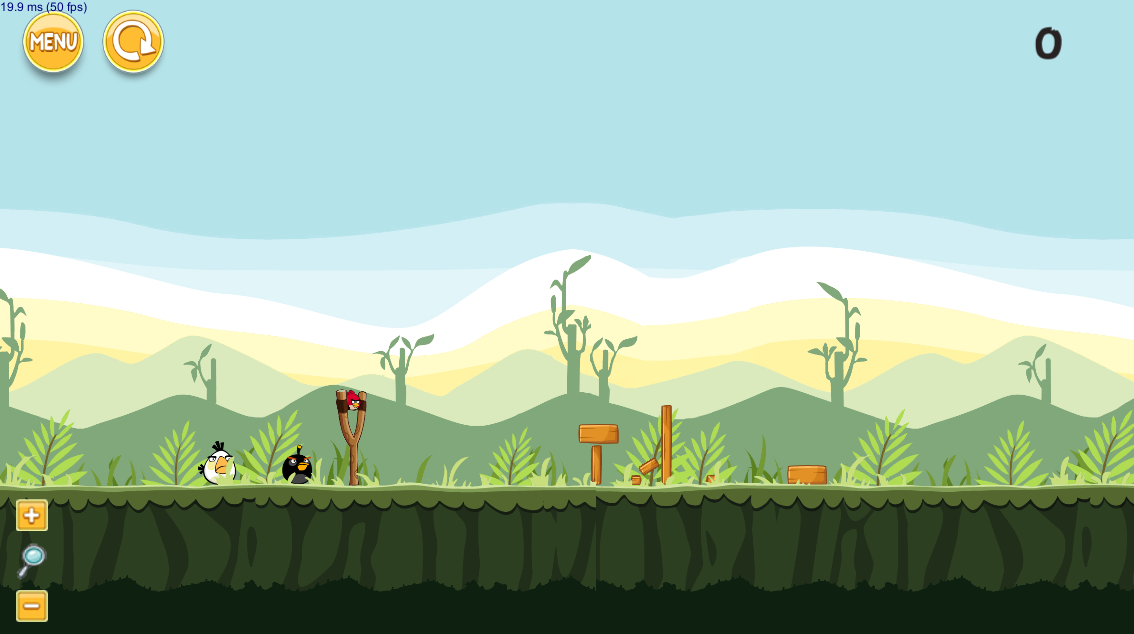
\includegraphics[scale=0.35]{gfx/e1/level-0-180522_171359.png}
	\caption{Fitness = 5.496, nBlocks = 9, G = 100 }\label{f:e1-1}
\end{figure}

\begin{figure}[H]
	\centering
	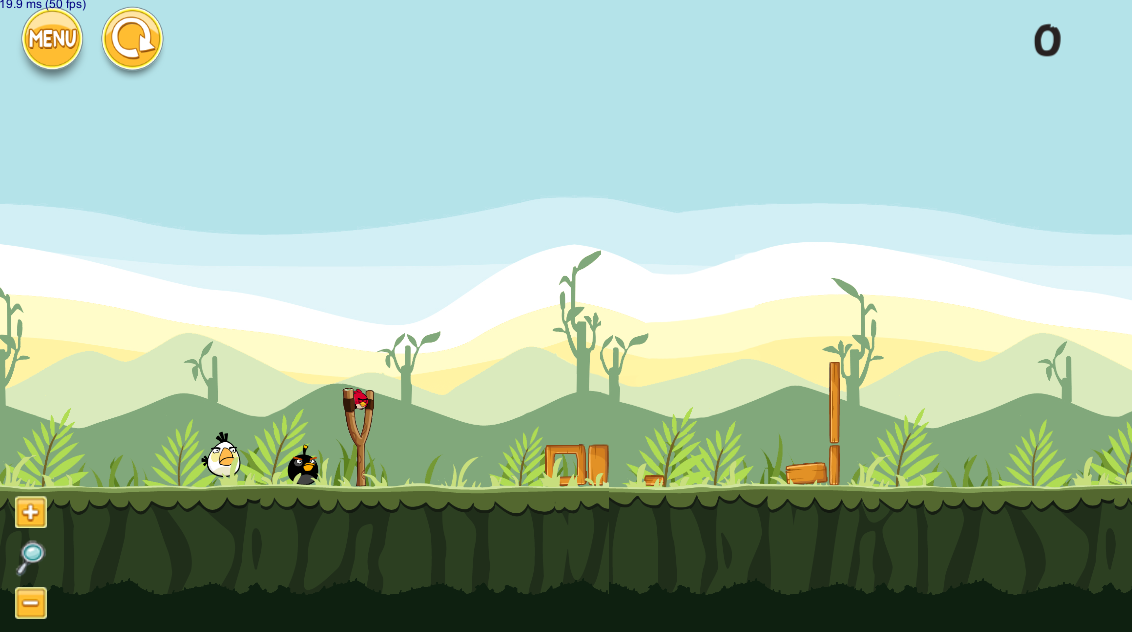
\includegraphics[scale=0.35]{gfx/e1/level-0-180522_183913.png}
	\caption{Fitness = 7.777, nBlocks = 8, G = 100 }\label{f:e1-2}
\end{figure}

\begin{figure}[H]
	\centering
	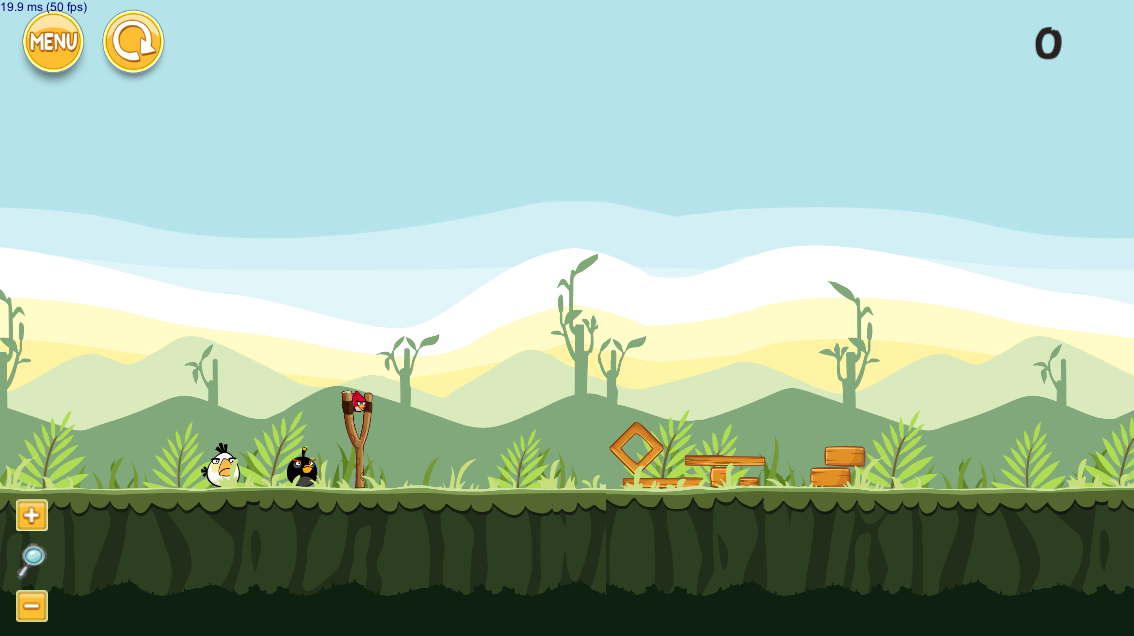
\includegraphics[scale=0.35]{gfx/e1/level-0-180523_194214.png}
	\caption{Fitness = 8.154, nBlocks = 7, G = 100 }\label{f:e1-3}
\end{figure}

\begin{figure}[H]
	\centering
	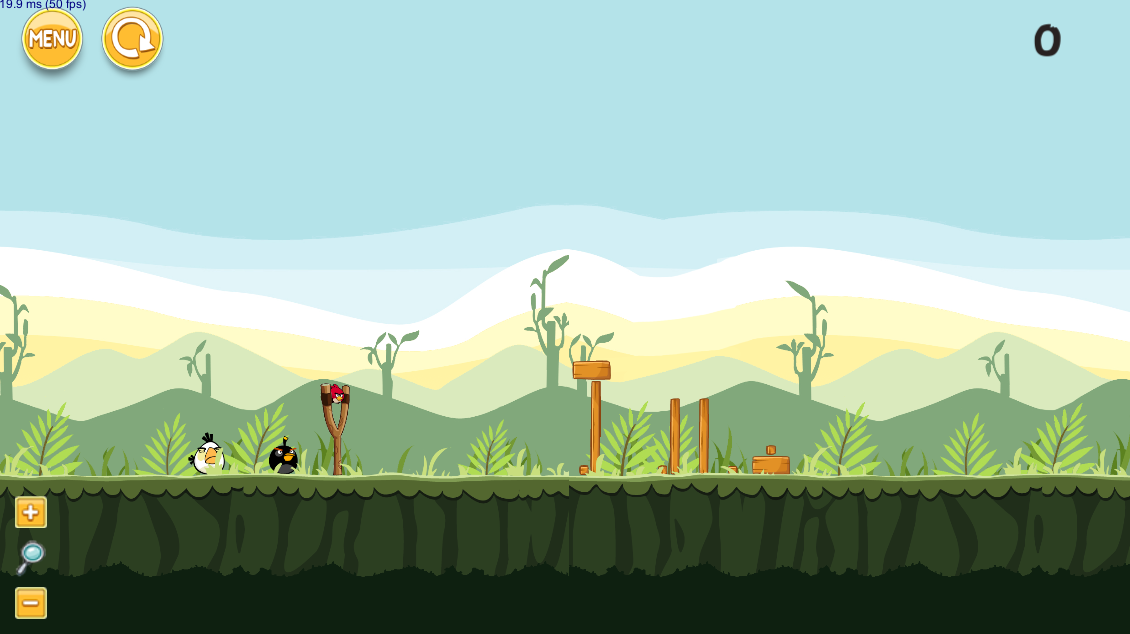
\includegraphics[scale=0.35]{gfx/e1//level-0-180523_203106.png}
	\caption{Fitness = 9.021, nBlocks = 7, G = 100  }\label{f:e1-4}
\end{figure}

\subsection{Experiment 2}\label{a:e2}

\begin{figure}[H]
	\centering
	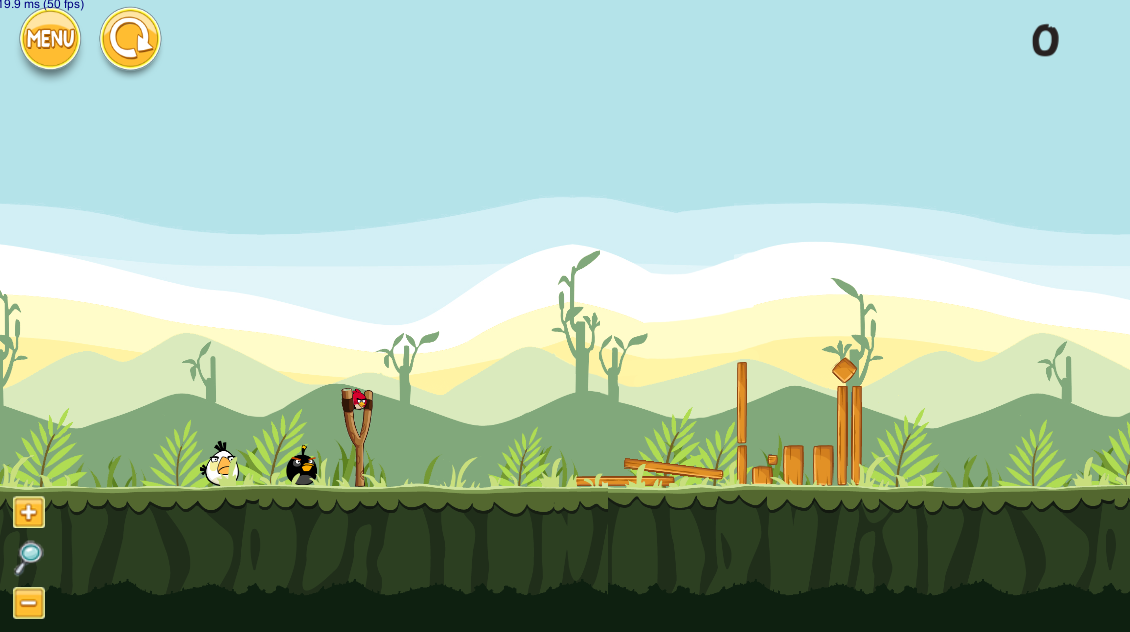
\includegraphics[scale=0.35]{gfx/e2/level-0-base_large180524_182751.png}
	\caption{Fitness = 5.276, nBlocks = 11, G = 383 }\label{f:e2-1}
\end{figure}

\begin{figure}[H]
	\centering
	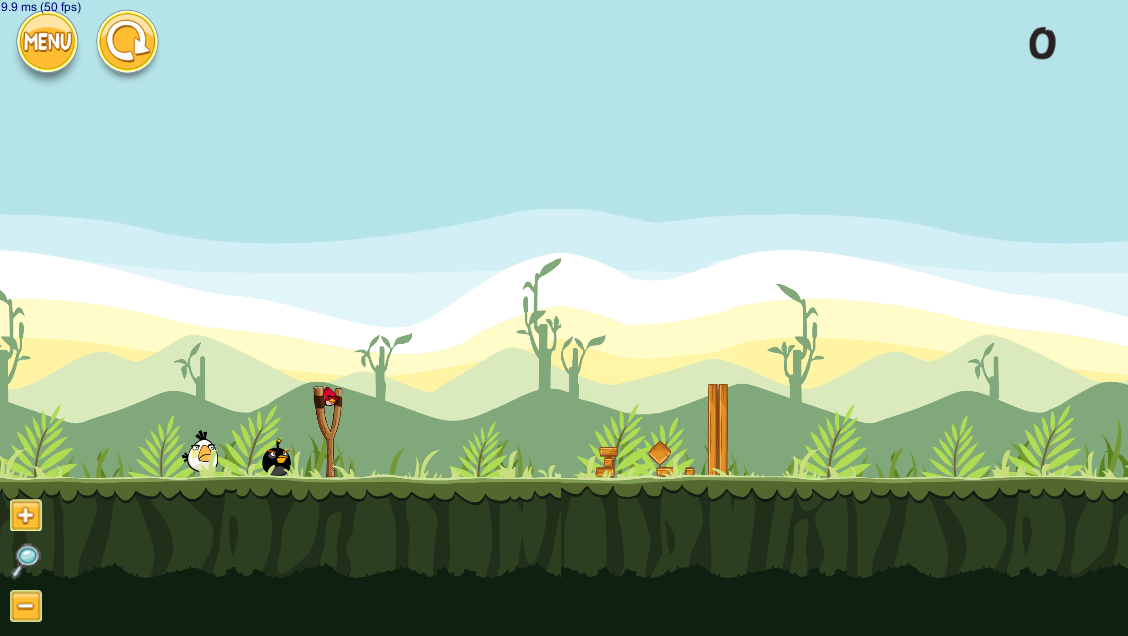
\includegraphics[scale=0.35]{gfx/e2/level-0-base_large180525_034217.png}
	\caption{Fitness = 2.909, nBlocks = 8, G = 364 }\label{f:e2-2}
\end{figure}

\begin{figure}[H]
	\centering
	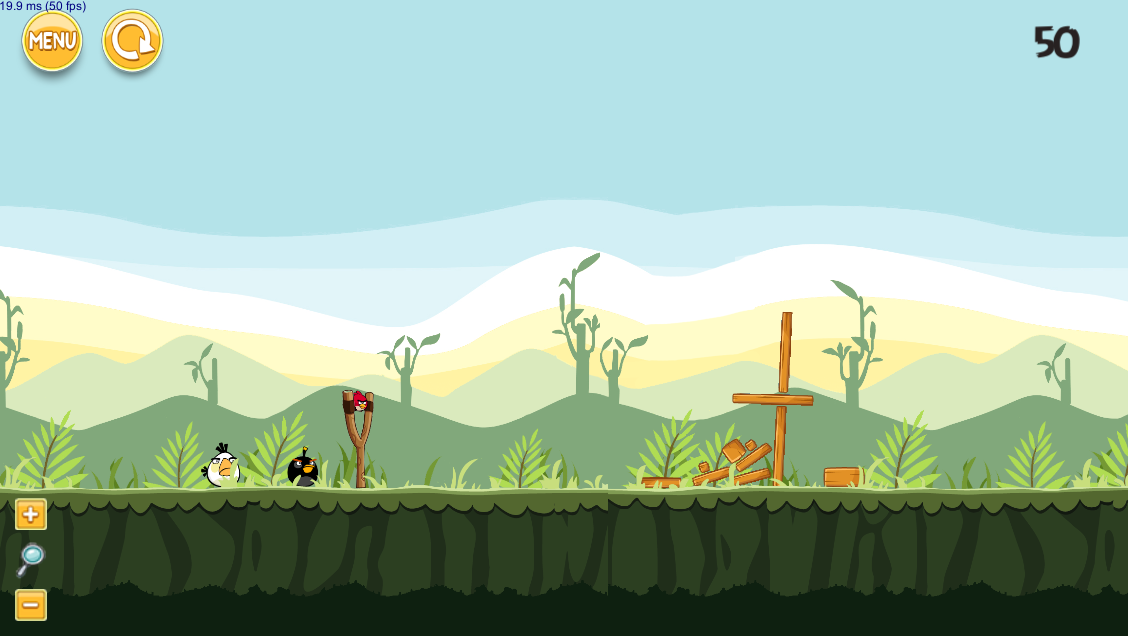
\includegraphics[scale=0.35]{gfx/e2/level-0-base_large180529_221751.png}
	\caption{Fitness = 203.776, nBlocks = 13, G = 44 }\label{f:e2-3}
\end{figure}

\begin{figure}[H]
	\centering
	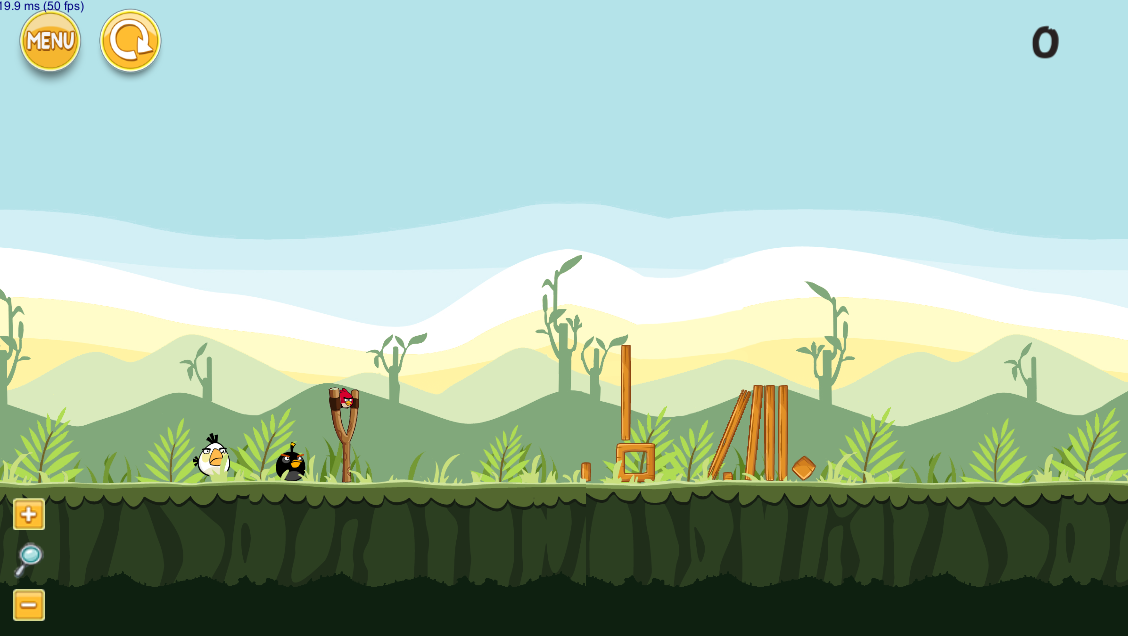
\includegraphics[scale=0.35]{gfx/e2/level-0-base_large180529_223045.png}
	\caption{Fitness = 5.176, nBlocks = 9, G = 767  }\label{f:e2-4}
\end{figure}

\subsection{Experiment 3}\label{a:e3}
\begin{figure}[H]
	\centering
	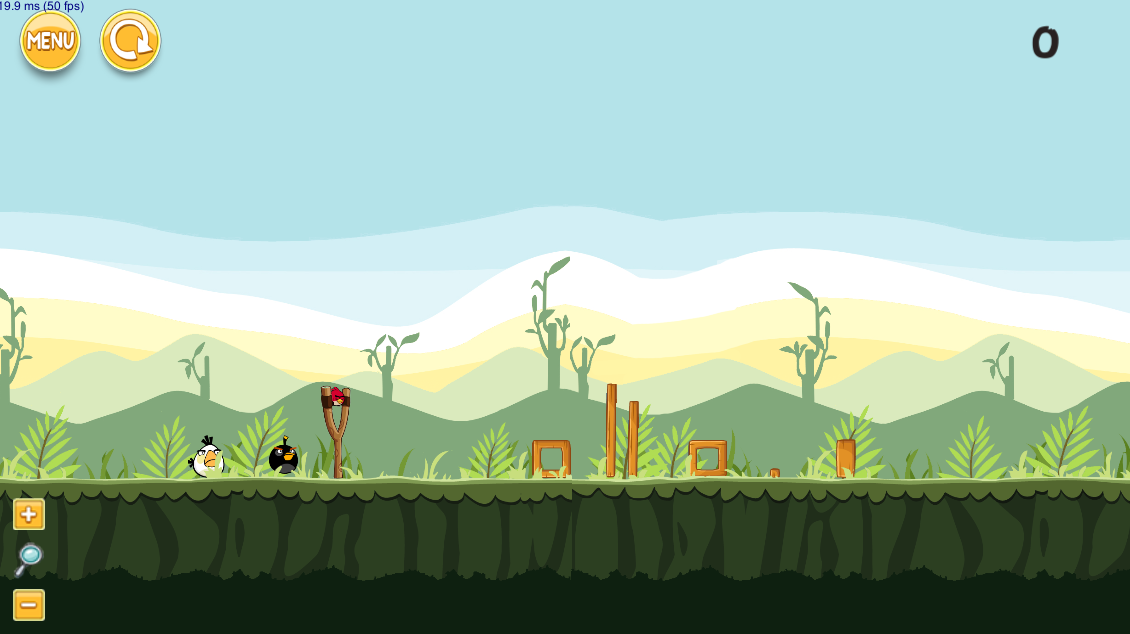
\includegraphics[scale=0.35]{gfx/e3/level-0-second_crossover180613_010758.png}
	\caption{Fitness = 8.334e-8, nBlocks = 6, G = 52 }\label{f:e3-1}
\end{figure}

\begin{figure}[H]
	\centering
	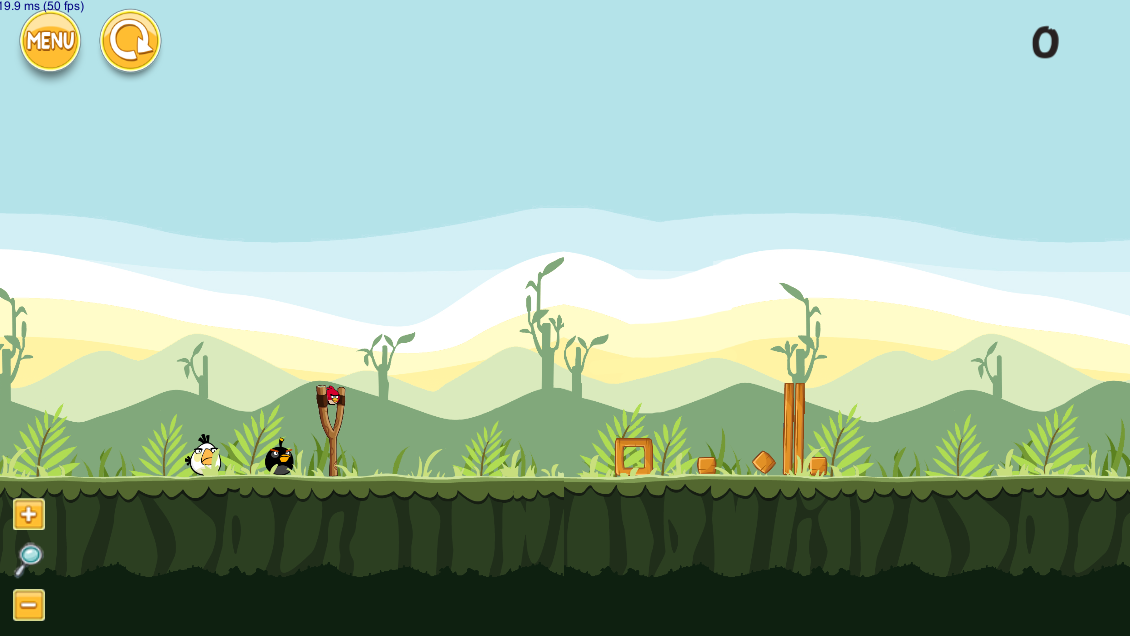
\includegraphics[scale=0.35]{gfx/e3/level-0-second_crossover180613_024124.png}
	\caption{Fitness = 6.035e-8, nBlocks = 6, G = 69 }\label{f:e3-2}
\end{figure}

\begin{figure}[H]
	\centering
	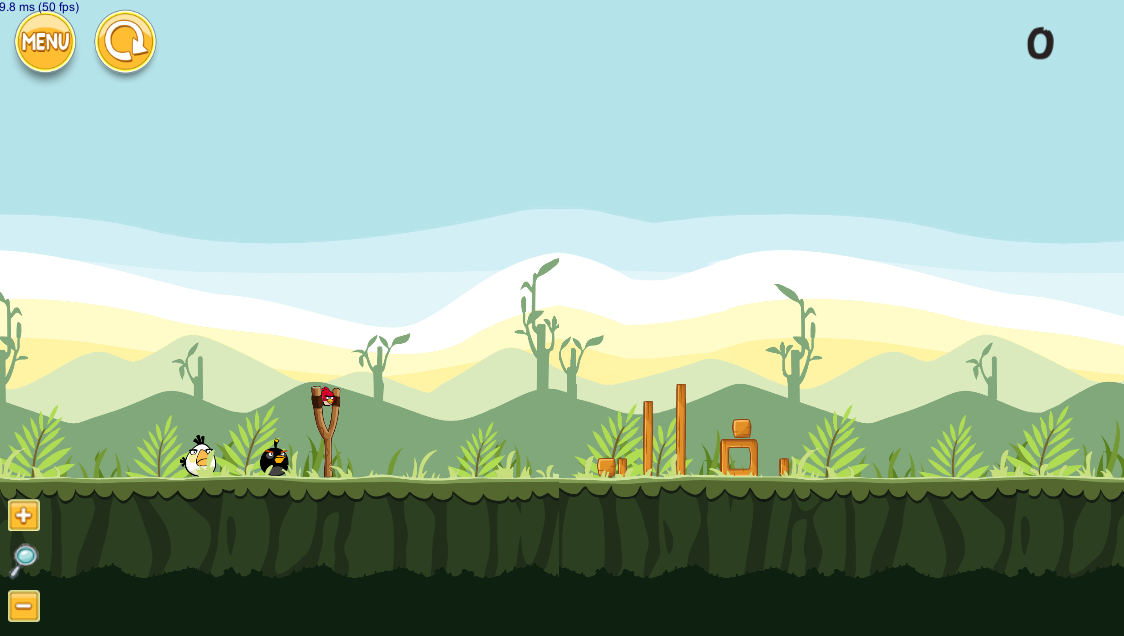
\includegraphics[scale=0.35]{gfx/e3/level-0-second_crossover180613_041716.png}
	\caption{Fitness = 9.856e-8, nBlocks = 7, G = 76 }\label{f:e3-3}
\end{figure}

\begin{figure}[H]
	\centering
	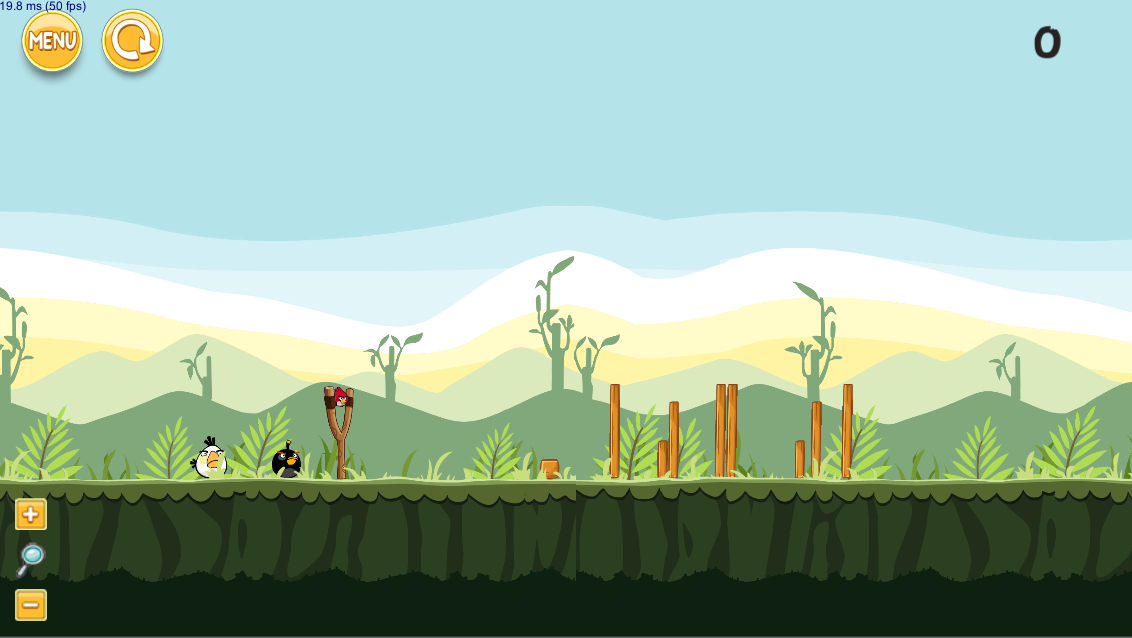
\includegraphics[scale=0.35]{gfx/e3/level-0-second_crossover180613_055622.png}
	\caption{Fitness = 1.571e-7, nBlocks = 9, G = 194  }\label{f:e3-4}
\end{figure}
\subsection{Experiment 4}\label{a:e4}

\begin{figure}[H]
	\centering
	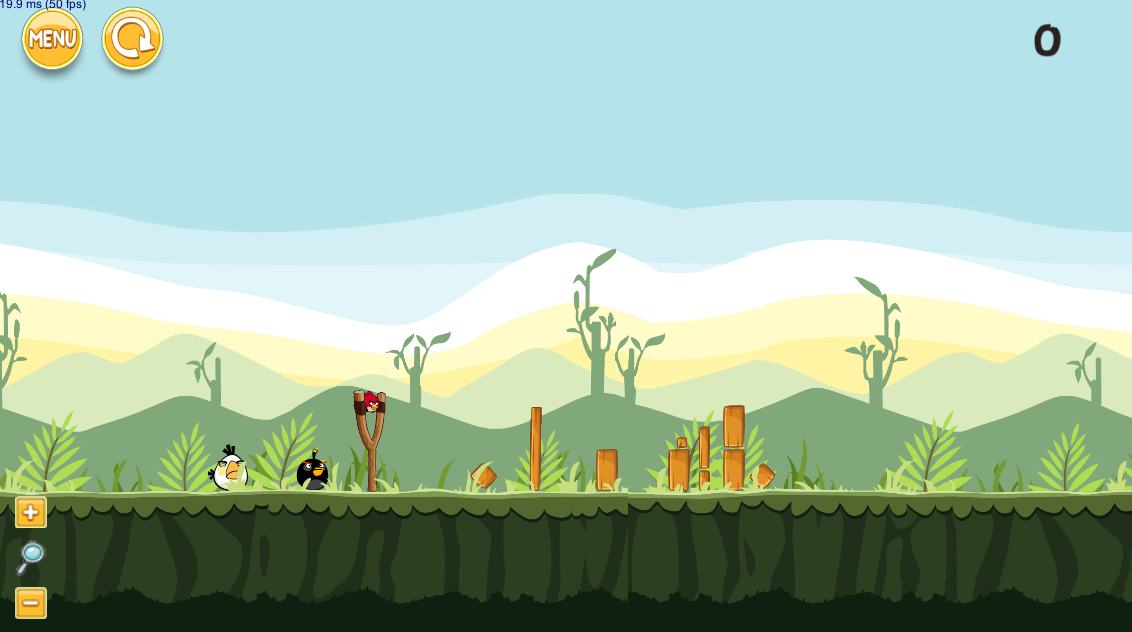
\includegraphics[scale=0.35]{gfx/e4/level-0-second_crossover_min10_180602_035405.png}
	\caption{Fitness = 9.229e-7, nBlocks = 10, G = 198 }\label{f:e4-1}
\end{figure}

\begin{figure}[H]
	\centering
	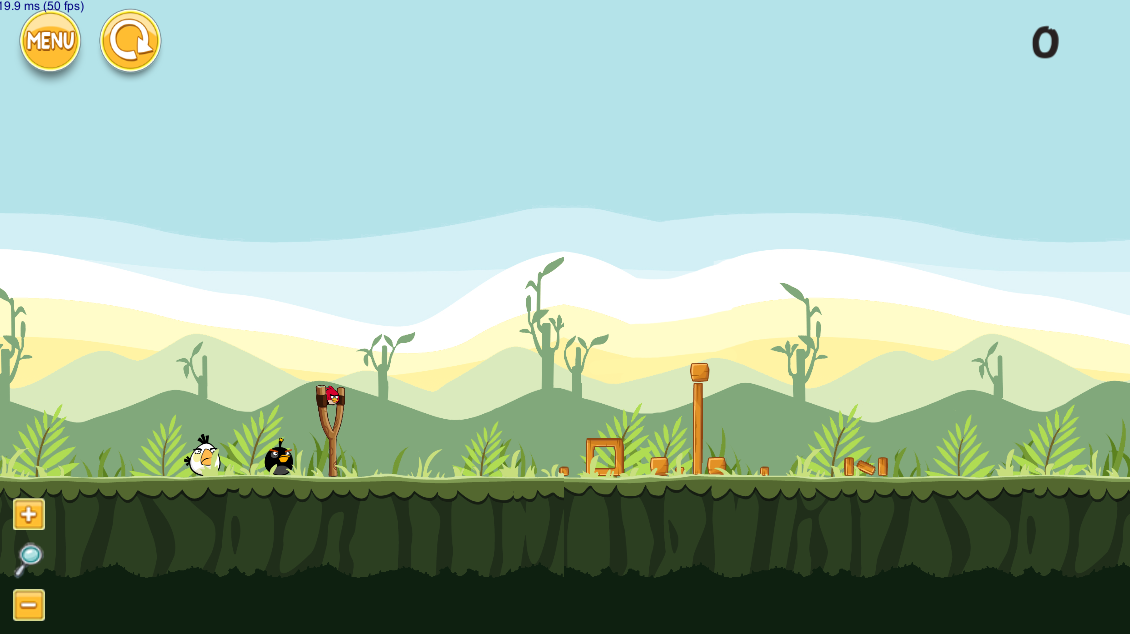
\includegraphics[scale=0.35]{gfx/e4/level-0-second_crossover_min10_180603_040806.png}
	\caption{Fitness = 1.065e-7, nBlocks = 11, G = 344 }\label{f:e4-2}
\end{figure}

\begin{figure}[H]
	\centering
	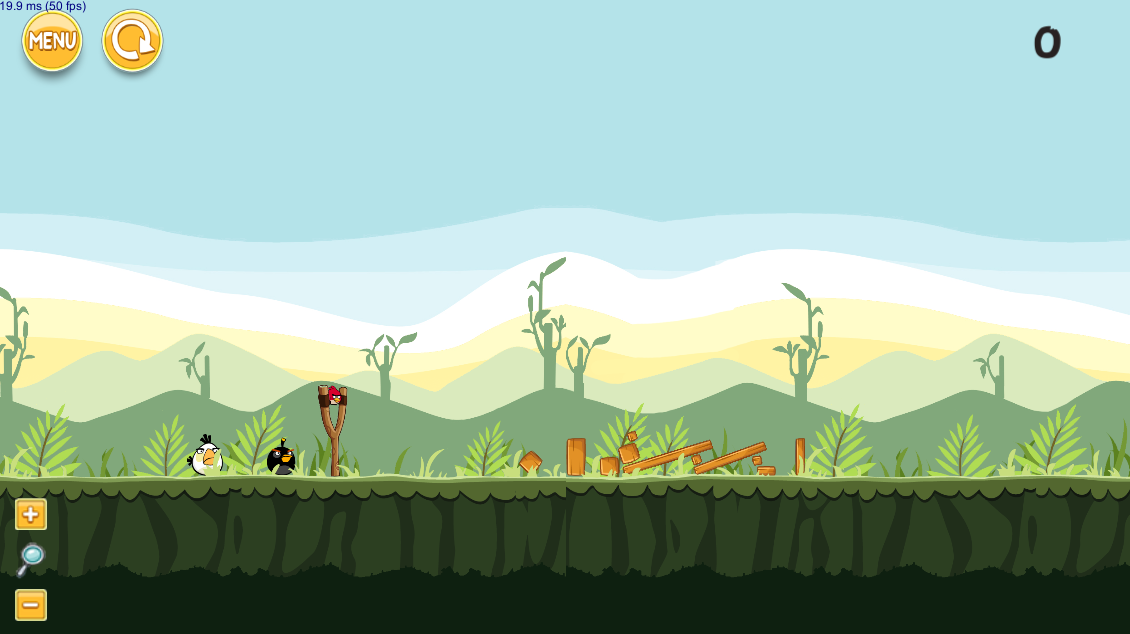
\includegraphics[scale=0.35]{gfx/e4/level-0-second_crossover_min10_180606_233100.png}
	\caption{Fitness = 8.395e-5, nBlocks = 11, G = 375 }\label{f:e4-3}
\end{figure}

\begin{figure}[H]
	\centering
	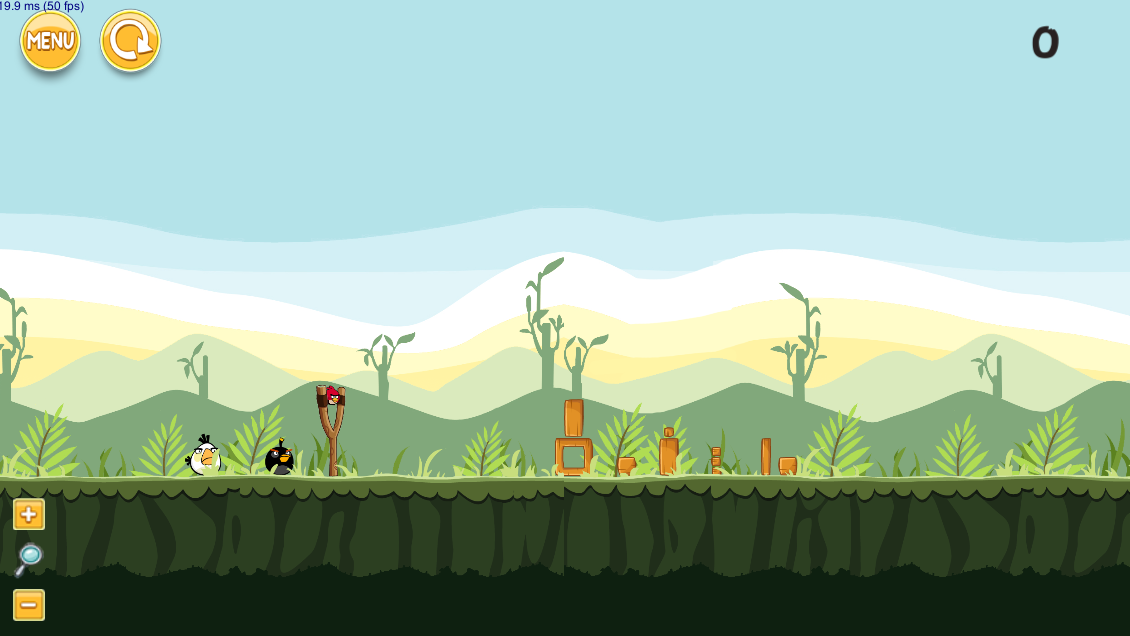
\includegraphics[scale=0.35]{gfx/e4/level-0-second_crossover_min10_verbose180614_181948.png}
	\caption{Fitness = 8.946e-6, nBlocks = 10, G = 320  }\label{f:e4-4}
\end{figure}


%*****************************************
%*****************************************
%*****************************************
%*****************************************
%*****************************************

%********************************************************************
% Other Stuff in the Back
%*******************************************************
\cleardoublepage%********************************************************************
% Bibliography
%*******************************************************
% work-around to have small caps also here in the headline
% https://tex.stackexchange.com/questions/188126/wrong-header-in-bibliography-classicthesis
% Thanks to Enrico Gregorio
\defbibheading{bibintoc}[\bibname]{%
  \phantomsection
  \manualmark
  \markboth{\spacedlowsmallcaps{#1}}{\spacedlowsmallcaps{#1}}%
  \addtocontents{toc}{\protect\vspace{\beforebibskip}}%
  \addcontentsline{toc}{chapter}{\tocEntry{#1}}%
  \chapter*{#1}%
}
\printbibliography[heading=bibintoc]

% Old version, will be removed later
% work-around to have small caps also here in the headline
%\manualmark
%\markboth{\spacedlowsmallcaps{\bibname}}{\spacedlowsmallcaps{\bibname}} % work-around to have small caps also
%\phantomsection
%\refstepcounter{dummy}
%\addtocontents{toc}{\protect\vspace{\beforebibskip}} % to have the bib a bit from the rest in the toc
%\addcontentsline{toc}{chapter}{\tocEntry{\bibname}}
%\label{app:bibliography}
%\printbibliography

\cleardoublepage%*******************************************************
% Declaration
%*******************************************************
\refstepcounter{dummy}
\pdfbookmark[0]{Declaration}{declaration}
\chapter*{Declaration}
\thispagestyle{empty}
\textbf{\MakeUppercase{\myName}} con DNI *, actuando en su propio nombre y derecho,

\bigskip

\textbf{DECLARA, BAJO SU RESPONSABILIDAD:}

\bigskip

Que el Trabajo Fin de Grado presentado en la \myFaculty de la \myUni, con fecha 18 de Junio de 2018, titulado \textit{\myTitle, \mySubtitle} es original, no es copia ni adaptación de ningún otro trabajo, inédito, y no ha sido difundido por ningún medio, ni presentado anteriormente por quien suscribe o por otra persona. 

\bigskip

Y para que así conste a los efectos oportunos, firmo la presente en \myLocation, a 18 de Junio de 2018. 

\smallskip

\begin{flushright}
	\begin{tabular}{m{5cm}}
		\\ \hline
		\centering\myName \\
	\end{tabular}
\end{flushright}

\bigskip

\bigskip

Yo, \myName, alumno del \myDegree de la \myFaculty de la \myUni con DNI *, autorizo la
ubicación de la siguiente copia de mi Trabajo Fin de Grado en la biblioteca del centro para que pueda ser
consultada por las personas que lo deseen.

\bigskip

\noindent\textit{\myLocation, \myTime}

\smallskip

\begin{flushright}
    \begin{tabular}{m{5cm}}
        \\ \hline
        \centering\myName \\
    \end{tabular}
\end{flushright}

\cleardoublepage\pagestyle{empty}

\hfill

\vfill


\pdfbookmark[0]{Colophon}{colophon}
\section*{Colophon}
This document was typeset using the typographical look-and-feel \texttt{classicthesis} developed by Andr\'e Miede and Ivo Pletikosić.
The style was inspired by Robert Bringhurst's seminal book on typography ``\emph{The Elements of Typographic Style}''.
\texttt{classicthesis} is available for both \LaTeX\ and \mLyX:
\begin{center}
\url{https://bitbucket.org/amiede/classicthesis/}
\end{center}
Happy users of \texttt{classicthesis} usually send a real postcard to the author, a collection of postcards received so far is featured here:
\begin{center}
\url{http://postcards.miede.de/}
\end{center}
Thank you very much for your feedback and contribution.

\bigskip

\noindent\finalVersionString

%Hermann Zapf's \emph{Palatino} and \emph{Euler} type faces (Type~1 PostScript fonts \emph{URW
%Palladio L} and \emph{FPL}) are used. The ``typewriter'' text is typeset in \emph{Bera Mono},
%originally developed by Bitstream, Inc. as ``Bitstream Vera''. (Type~1 PostScript fonts were made
%available by Malte Rosenau and
%Ulrich Dirr.)

%\paragraph{note:} The custom size of the textblock was calculated
%using the directions given by Mr. Bringhurst (pages 26--29 and
%175/176). 10~pt Palatino needs  133.21~pt for the string
%``abcdefghijklmnopqrstuvwxyz''. This yields a good line length between
%24--26~pc (288--312~pt). Using a ``\emph{double square textblock}''
%with a 1:2 ratio this results in a textblock of 312:624~pt (which
%includes the headline in this design). A good alternative would be the
%``\emph{golden section textblock}'' with a ratio of 1:1.62, here
%312:505.44~pt. For comparison, \texttt{DIV9} of the \texttt{typearea}
%package results in a line length of 389~pt (32.4~pc), which is by far
%too long. However, this information will only be of interest for
%hardcore pseudo-typographers like me.%
%
%To make your own calculations, use the following commands and look up
%the corresponding lengths in the book:
%\begin{verbatim}
%    \settowidth{\abcd}{abcdefghijklmnopqrstuvwxyz}
%    \the\abcd\ % prints the value of the length
%\end{verbatim}
%Please see the file \texttt{classicthesis.sty} for some precalculated
%values for Palatino and Minion.
%
%    \settowidth{\abcd}{abcdefghijklmnopqrstuvwxyz}
%    \the\abcd\ % prints the value of the length

% ********************************************************************
% Game Over: Restore, Restart, or Quit?
%*******************************************************
\end{document}
% ********************************************************************
